\documentclass[table, t,13pt]{beamer} 
\usepackage{graphicx}
\usepackage{xeCJK,fontspec,xunicode,xltxtra, fancybox}

%\usepackage[timeinterval=1]{tdclock}
%box tools
\usepackage{framed, color}
\usepackage{colortbl, booktabs, multirow, makecell, longtable}
\usepackage{tcolorbox}

\usepackage{soul} %for strikeout

\usepackage{amsmath, amsfonts, amssymb} %amssymb for varnothing symbol

\usepackage{caption, algorithm}
\usepackage[noend]{algpseudocode}

\usepackage{textpos}
\usepackage{tikz, flowchart} % tikz绘图
\usetikzlibrary{decorations.pathreplacing}
\usetikzlibrary{decorations.markings}
\usetikzlibrary{calc, arrows, arrows.meta, shapes, shapes.geometric, positioning}
\usetikzlibrary{topaths}
\usetikzlibrary{mindmap}
\usetikzlibrary{matrix}
\pgfmathsetmacro{\myinnersep}{2}% inner sep in mm
\tikzset{
%    box/.style={draw,%
%        inner sep=\myinnersep,%
%        outer sep=0,%
%    minimum width=5mm,%
%    minimum height=\heightof{Cap}+2*\myinnersep*1mm,%
%    align=center},
    database/.style={
      cylinder,
      cylinder uses custom fill,
      %cylinder body fill=green!5,
      %cylinder end fill=green!5,
      shape border rotate=90,
      aspect=0.25,
      inner sep=0.2cm,
      draw
    },
  multidocument/.style={
    shape=tape,
    draw,
    fill=white,
    tape bend top=none,
    double copy shadow},
  manual input/.style={
    shape=trapezium,
    draw,
    shape border rotate=90,
    trapezium left angle=90,
    trapezium right angle=80}
}


\makeatletter
\pgfdeclareshape{document}{
	\inheritsavedanchors[from=rectangle] % this is nearly a rectangle
	\inheritanchorborder[from=rectangle]
	\inheritanchor[from=rectangle]{center}
	\inheritanchor[from=rectangle]{north}
	\inheritanchor[from=rectangle]{south}
	\inheritanchor[from=rectangle]{west}
	\inheritanchor[from=rectangle]{east}
	% ... and possibly more
	\backgroundpath{% this is new
		% store lower right in xa/ya and upper right in xb/yb
		\southwest \pgf@xa=\pgf@x \pgf@ya=\pgf@y
		\northeast \pgf@xb=\pgf@x \pgf@yb=\pgf@y
		% compute corner of ‘‘flipped page’’
		\pgf@xc=\pgf@xb \advance\pgf@xc by-10pt % this should be a parameter
		\pgf@yc=\pgf@yb \advance\pgf@yc by-10pt
		% construct main path
		\pgfpathmoveto{\pgfpoint{\pgf@xa}{\pgf@ya}}
		\pgfpathlineto{\pgfpoint{\pgf@xa}{\pgf@yb}}
		\pgfpathlineto{\pgfpoint{\pgf@xc}{\pgf@yb}}
		\pgfpathlineto{\pgfpoint{\pgf@xb}{\pgf@yc}}
		\pgfpathlineto{\pgfpoint{\pgf@xb}{\pgf@ya}}
		\pgfpathclose
		% add little corner
		\pgfpathmoveto{\pgfpoint{\pgf@xc}{\pgf@yb}}
		\pgfpathlineto{\pgfpoint{\pgf@xc}{\pgf@yc}}
		\pgfpathlineto{\pgfpoint{\pgf@xb}{\pgf@yc}}
		\pgfpathlineto{\pgfpoint{\pgf@xc}{\pgf@yc}}
	}
}
\makeatother

\newcommand{\Simley}[3]{%
\begin{tikzpicture}[scale=0.11]
    \newcommand*{\SmileyRadius}{#2}%
    \draw [fill=brown!10] (0,0) circle (\SmileyRadius)% outside circle
        %node [yshift=-0.22*\SmileyRadius cm] {\tiny #1}% uncomment this to see the smile factor
        ;  

    \pgfmathsetmacro{\eyeX}{0.5*\SmileyRadius*cos(30)}
    \pgfmathsetmacro{\eyeY}{0.5*\SmileyRadius*sin(30)}
    \draw [fill=cyan,draw=none] (\eyeX,\eyeY) circle (#3 cm);
    \draw [fill=cyan,draw=none] (-\eyeX,\eyeY) circle (#3 cm);

    \pgfmathsetmacro{\xScale}{2*\eyeX/180}
    \pgfmathsetmacro{\yScale}{1.0*\eyeY}
    \draw[color=red, domain=-\eyeX:\eyeX]   
        plot ({\x},{
            -0.1+#1*0.15 % shift the smiley as smile decreases
            -#1*1.75*\yScale*(sin((\x+\eyeX)/\xScale))-\eyeY});
\end{tikzpicture}%
}%
%  \Simley{1}{10}{1}
%  \Simley{0.5}{10}{1}
%  \Simley{0}{10}{1}
%  \Simley{-0.5}{10}{1}
%  \Simley{-1}{10}{1}


\usepackage{pgfplots}
\usepgfplotslibrary{external}  %缓存tikz的结果
\tikzset{
    external/system call={%
    xelatex \tikzexternalcheckshellescape
    -halt-on-error -interaction=batchmode --shell-escape
    -jobname "\image" "\texsource"}}
%\tikzexternalize


\usepackage[tikz]{bclogo}  %see http://mirrors.ctan.org/graphics/bclogo/README
\DeclareGraphicsRule{.mps}{eps}{*}{} %解决xelatex处理bclogo时的mps问题
\newcommand{\infobox}[2]{ 
    \begin{bclogo}[couleur=yellow!10, logo=\bcfleur, ombre=true]{#1}
    #2
    \end{bclogo}
}
\newcommand{\warnbox}[2]{ 
    \begin{bclogo}[couleur=yellow!10, logo=\bctakecare, ombre=true]{#1}
    #2
    \end{bclogo}
}
\newcommand{\kpt}{{\color{red}$\ast$}}
\newcommand{\h}{{\color{orange!70}$\bullet ~ $}}
\newcommand{\hh}{{\color{orange!70}$~~ \ast ~ $}}

\newcommand{\newsec}{\color{red} $\Rightarrow$}

%\usetheme[height=8mm]{Madrid} % Favorite theme is Madrid! 
%\usecolortheme[RGB={130,120,232}]{structure} 
%\usetheme{Boadilla} 
%\usecolortheme{default} 

\usetheme{Madrid} 
\usecolortheme{crane} 

\setbeamertemplate{items}[ball] 
\setbeamertemplate{blocks}[rounded][shadow=true] 

\definecolor{red(ncs)}{rgb}{0.77, 0.01, 0.2}
\definecolor{champagne}{rgb}{0.97, 0.91, 0.81}
\definecolor{coolblack}{rgb}{0.0, 0.18, 0.39}
\definecolor{vanilla}{rgb}{0.95, 0.9, 0.67}

\usepackage[ampersand]{easylist}
\newcommand\easyitem{\ListProperties(Hide=100, Hang=true, Progressive=3ex,
  Style*=\color{orange!70}$\bullet$ ,
  Style2*=\color{orange!70}$\ast$ ,
  Style3*=\color{orange!70}$\circ$ ,
  Style4*=\tiny$\blacksquare$, Space=-.5em, Space*=-.5em)}

\parskip=3mm
\parindent=15pt
\linespread{1.1}


%自定义的一些命令,方便使用
\newcommand*\circled[1]{\tikz[baseline=(char.base)]{
  \node[shape=circle,draw,inner sep=1.5pt] (char) {#1};}}


% \newcommand*{\hei}{\fontfamily{FZLanTingHeiS-H-GB}\selectfont}
%\DeclareTextFontCommand{\texthei}{\hei}

\setCJKfamilyfont{FZHei}{FZLanTingHeiS-EL-GB}  
\newcommand{\cjkbold}{\color[rgb]{0.29, 0.0, 0.51} \CJKfamily{FZHei}}  %http://latexcolor.com/

\setCJKmainfont{FZLanTingHeiS-EL-GB} %方正字体,也可以改成:微软雅黑
\setCJKsansfont{FZLanTingHeiS-EL-GB} 
\setCJKmonofont{Consolas}


% % 设置英文字体%==================================================
%\defaultfontfeatures{Scale=MatchLowercase} % 这个参数保证 serif、sans-serif 和
% %monospace 字体在小写时大小匹配
%\setmainfont[Mapping=tex-text]{Ubuntu} % 使用 XeTeX 的 text-mapping 方案,正确显示 LaTeX 样式的双引号(`` '')%

%\setsansfont[Mapping=tex-text]{Consolas}
%\setmonofont{Ubuntu Light}

% FONTS
\defaultfontfeatures{Mapping=tex-text}
\setsansfont[  %\setmainfont[
SmallCapsFont = Fontin-SmallCaps.otf,
BoldFont = Fontin-Bold.otf,
ItalicFont = Fontin-Italic.otf
]
{Fontin.otf}



\newcommand{\cjkem}{\CJKfamily{FZHeiR}} 
\renewcommand{\em}[1]{\color{red} #1}

\XeTeXlinebreaklocale "zh"  
\XeTeXlinebreakskip = 0pt plus 1pt 

\usepackage{listings,lstautogobble}
\lstset{breakatwhitespace,
backgroundcolor=\color{white},
columns=fullflexible,
breaklines,
showtabs=true,
tabsize=4,
keepspaces=true,
keywordstyle=\color{blue},
extendedchars=true,
basicstyle=\rmfamily\normalsize, 
prebreak=, %
autogobble=true, 
keywordstyle=\ttfamily, 
numberstyle=\tiny\color{green!70}\ttfamily}

% Definition of JavaScript
\definecolor{lightgray}{rgb}{.9,.9,.9}
\definecolor{darkgray}{rgb}{.4,.4,.4}
\definecolor{purple}{rgb}{0.65, 0.12, 0.82}

\lstdefinelanguage{JavaScript}{
  keywords={typeof, new, true, false, catch, function, return, null, catch, switch, var, if, in, while, do, else, case, break},
  keywordstyle=\color{blue}\bfseries,
  ndkeywords={class, export, boolean, throw, implements, import, this},
  ndkeywordstyle=\color{darkgray}\bfseries,
  identifierstyle=\color{black},
  sensitive=false,
  comment=[l]{//},
  morecomment=[s]{/*}{*/},
  commentstyle=\color{purple}\ttfamily,
  stringstyle=\color{red}\ttfamily,
  morestring=[b]',
  morestring=[b]"
}

\lstset{
   language=JavaScript,
   %backgroundcolor=\color{lightgray},
   extendedchars=true,
   basicstyle=\footnotesize\ttfamily,
   showstringspaces=false,
   showspaces=false,
   numbers=left,
   numberstyle=\footnotesize,
   numbersep=9pt,
   tabsize=2,
   breaklines=true,
   showtabs=false,
   captionpos=t
}


% Definition of CSS
\definecolor{lightgray}{rgb}{0.95, 0.95, 0.95}
\definecolor{darkgray}{rgb}{0.4, 0.4, 0.4}
\definecolor{purple}{rgb}{0.65, 0.12, 0.82}

\lstdefinelanguage{CSS}{
    keywords={color,background-image,margin,padding,font,weight,display,position,top,left,right,bottom,list,style,border,size,white,space,min,width, transform, transition, transition-property, transition-duration, transition-timing-function},
    alsodigit={-},
    sensitive=true,
    morecomment=[l]{//},
    morecomment=[s]{/*}{*/},
    morestring=[b]',
    morestring=[b]"
}

\lstset{%
    % General design
    %backgroundcolor=\color{lightgray},
    basicstyle={\small\ttfamily},   
    frame=l,
    % Code design
    identifierstyle=\color{black},
    keywordstyle=\color{blue}\bfseries,
    %ndkeywordstyle=\color{green}\bfseries,
    stringstyle=\color{ocherCode}\ttfamily,
    commentstyle=\color{darkgray}\ttfamily,
    % Code
    language={CSS},
    tabsize=2,
    showtabs=false,
    showspaces=false,
    showstringspaces=false,
    extendedchars=true,
    breaklines=true,
    % line-numbers
    xleftmargin={0.75cm},
    numbers=left,
    stepnumber=1,
    firstnumber=1,
    numberfirstline=true,
}


\definecolor{orangered}{RGB}{239,134,64}
\definecolor{tagcolor}{RGB}{0,0,150}
\definecolor{keywordcolor}{RGB}{139,38,201}
\definecolor{attr_value_color}{RGB}{153,51,0}

\lstset{
    language=XML,
    tabsize=4,
    %caption=Code,
    label=code:sample,
    frame=shadowbox,
    rulesepcolor=\color{gray},
    xleftmargin=20pt,
    framexleftmargin=15pt,
    keywordstyle=\color{keywordcolor}\bf,
    commentstyle=\color{gray},
    stringstyle=\color{attr_value_color},    
    tagstyle=\color{tagcolor}\bf,
    markfirstintag=\color{red}\bf,
    numbers=left,
    numberstyle=\tiny,
    numbersep=5pt,
    breaklines=true,
    showstringspaces=false,
    basicstyle=\footnotesize,
    morekeywords={xmlns,version,type,encoding,xml-stylesheet, xs:schema,xs:element,xs:complexType,xs:sequence,xs:attribute}, % list your attributes here
    emphstyle={\color{blue}}}
\renewcommand{\lstlistingname}{Code}

%%% Local Variables:
%%% mode: latex
%%% TeX-master: t
%%% End:


\lstnewenvironment{python}{\renewcommand\lstlistingname{Python} %
\lstset{language=python,basicstyle=\rmfamily\normalsize, prebreak=, %
  autogobble=true, keywordstyle=\ttfamily, %
  escapechar=|,
  numberstyle=\tiny\color{orange!90}\ttfamily, showstringspaces=false} } %
{}

\lstnewenvironment{bash}{\renewcommand\lstlistingname{Bash} %
\lstset{language=bash,basicstyle=\rmfamily\normalsize, prebreak=, %
  autogobble=true, keywordstyle=\ttfamily, numberstyle=\tiny\color{green!70}\ttfamily}} %
{}

\newcommand{\pyinline}[1]{\small{\color{blue!50!green}$>>>$}
  \lstinline[language=python, basicstyle=\rmfamily\normalsize, keywordstyle={\ttfamily\color{blue!50!black}}]!#1!}

\hypersetup{
  pdftitle={Python程序设计},
  pdfsubject={Python},
  pdfkeywords={Python},
  pdfproducer={LaTeX},
  pdfcreator={XeLaTeX}
}


%\setbeamercolor{title}{bg=red(ncs), fg=white}
%\setbeamercolor{frametitle}{fg=red(ncs),bg=gray!10!white}
\setbeamercolor{title}{fg=coolblack, bg=vanilla}
\setbeamercolor{frametitle}{fg=coolblack, bg=vanilla!0}

\setbeamercolor{palette primary}{fg=black, bg=gray!15!white}
\setbeamercolor{palette secondary}{fg=black, bg=gray!10!white}
\setbeamercolor{palette tertiary}{fg=black, bg=gray!15!white}


\addtobeamertemplate{frametitle}{}{%
\begin{textblock*}{1.0\paperwidth}(-.001\textwidth,0cm)
%\tikz{\draw[orange!95, line width=1.1] (-2cm,0cm) -- (0.5\textwidth,0cm);\draw[orange!95,yshift=-0.55] (0.5\textwidth,0cm) -- (0.7\textwidth,0cm);}
\end{textblock*}
\begin{textblock*}{100mm}(.88\textwidth,-1cm)

\includegraphics[height=1.2cm,width=1.2cm]{ruc_logo.png}
\end{textblock*}
}

%gets rid of bottom navigation bars
\setbeamertemplate{footline}[page number]{}

%gets rid of navigation symbols
\setbeamertemplate{navigation symbols}{}

\setbeamercolor{item projected}{bg=orange!70!orange,fg=white}
\setbeamertemplate{enumerate items}[circle]

\begin{document}

%\logo{\includegraphics[width=1.0cm,height=1.0cm]{figure/ruc.jpg}}
\title{Python程序设计}
\author{Xia Tian \\ Email: xiat(at)ruc.edu.cn}
\institute{Renmin University of China}
\date{\today{}}
%\date[\initclock\tdtime]{\today}  
\frame{\titlepage}

%\begin{frame}[fragile]{整体内容}
  \begin{easylist} \easyitem
    & 简介
    & 数据类型
    & 控制流
    & 函数
    & 模块
    & 标准库
    & 面向对象编程
    & 异常、调试与测试
    & 输入输出
    & 应用(Web, DB, etc.)
  \end{easylist}
\end{frame}


\begin{frame}[fragile]{致谢}
  \begin{easylist}
    & 本课件的制作参考了部分图书和第三方网络资源,在此对原作者表达致谢和敬意,如
    有侵权需要从本课件中移除,请留言或联系xiat(at)ruc.edu.cn。参考资料包括但不限
    于以下:
    && 廖雪峰,
    \href{http://www.liaoxuefeng.com/wiki/0014316089557264a6b348958f449949df42a6d3a2e542c000}{Python教程}
    && Introducing Python by Bill Lubanovic
    && Dive Into Python 3 by Mark Pilgrim
    && Magnus Lie Hetland, 司维等翻译,Python基础教程(2ed), 人民邮电出版社
    && NumPy Cookbook
    && Python for Data Analysis
  \end{easylist}

\end{frame}

\section{引论}

\begin{frame}[fragile]{CH1 简介}
  \begin{easylist} \easyitem
    & 1.1 什么是Python
    & 1.2 Python可以做什么
    & 1.3 如何安装Python
    & 1.4 Python开发环境
    & 1.5 如何运行Python程序
    & 1.6 若干例子
  \end{easylist}
\end{frame}

\begin{frame}[fragile]{You're flying!}
  \begin{center}
    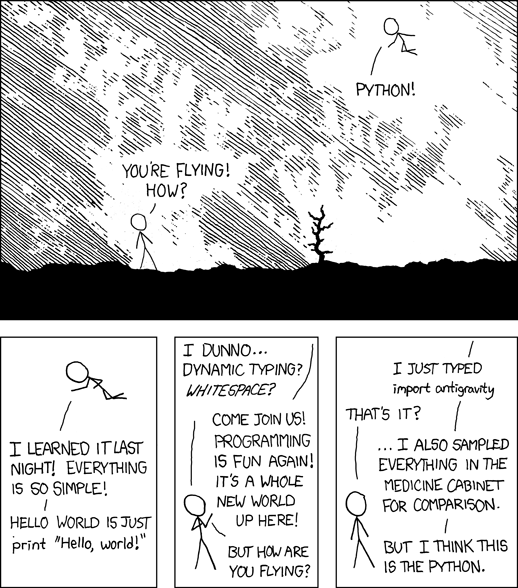
\includegraphics[height=0.9\textheight]{figure/fly.jpg}
  \end{center}
\end{frame}

\begin{frame}[fragile]{用Python,飞一般的感觉!}
  \begin{easylist}
    & \color{red} Friend :“你在飞!怎么做到的?”
    & Cueball:“Python!我昨晚刚刚学会了Python。一切都变得如此简单!写一个Hello World 程序只要一行代码 print "Hello World!" 就搞定了!”
    & \color{red}Friend :“ 什么情况?呃……动态类型?泛空格符?”
    & Cueball:“来加入我们吧,有了Python,编程再次变得有趣。这是一个全新的世界!”
    & \color{red}Friend :“但是你到底是怎么飞在天上的?”
    & Cueball:“我只是输入了“import antigravity” 命令而已。”
    & \color{red}Friend :“就这样?”
    & Cueball:“我还把药柜中的药嗑了个遍……但我觉得还是 Python 的原因。”
  \end{easylist}
\end{frame}

\begin{frame}[fragile]{1.1 什么是Python}
  \begin{easylist}
    & Python是一种既简单又强大的编程语言
    & 注重如何解决问题,而不是编程语言的语法和结构
    & 拥有高效的高级数据结构,简单有效地实现面向对象编程
    & 语法简洁、动态解释、适用于快速应用开发和脚本编程
    & 在数据科学中大有用武之地
  \end{easylist}
\end{frame}

\begin{frame}[plain]{}
  \begin{tikzpicture}[remember picture,overlay]
    \node[xshift=-60, yshift=-60] at (current page.north east) {
\includegraphics[]{figure/tim.png} };
  \end{tikzpicture}

  \LARGE The Zen of Python, \small by Tim Peters

  \normalsize 
  Beautiful is better than ugly. \\
  Explicit is better than implicit. \\
  Simple is better than complex. \\
  Complex is better than complicated. \\
  Flat is better than nested. \\
  Sparse is better than dense. \\
  Readability counts. \\
  Special cases aren't special enough to break the rules. \\
  Although practicality beats purity. \\
  Errors should never pass silently. \\
  Unless explicitly silenced.\\
  In the face of ambiguity, refuse the temptation to guess.\\
  There should be one-- and preferably only one --obvious way to do it.\\
  Although that way may not be obvious at first unless you're Dutch.\\
  Now is better than never.\\
  Although never is often better than *right* now.\\
  If the implementation is hard to explain, it's a bad idea.\\
  If the implementation is easy to explain, it may be a good idea.\\
  Namespaces are one honking great idea -- let's do more of those!\\
\end{frame}

\begin{frame}[plain]{}
  \begin{tikzpicture}[remember picture,overlay]
    \node[xshift=-60, yshift=-60] at (current page.north east) {
\includegraphics[]{figure/tim.png} };
  \end{tikzpicture}

  \LARGE Python之禅 \small by Tim Peters

  \normalsize
  优美胜于丑陋 \\ {\tiny Python 以编写优美的代码为目标}\\
  明了胜于晦涩 \\ {\tiny 优美的代码应当是明了的,命名规范,风格相似}\\
  简洁胜于复杂 \\ {\tiny 优美的代码应当是简洁的,不要有复杂的内部实现}\\
  复杂胜于凌乱 \\ {\tiny 如果复杂不可避免,那代码间也不能有难懂的关系,要保持接口简洁}\\
  扁平胜于嵌套 \\ {\tiny 优美的代码应当是扁平的,不能有太多的嵌套}\\
  间隔胜于紧凑 \\ {\tiny 优美的代码有适当的间隔,不要奢望一行代码解决问题}\\
  可读性很重要 \\ {\tiny 优美的代码是可读的}\\
  即便假借特例的实用性之名,也不可违背这些规则 \\ {\tiny 这些规则至高无上} \\
  不要包容所有错误,除非你确定需要这样做 \\ {\tiny 精准地捕获异常,不写 except:pass 风格的代码}\\
  当存在多种可能,不要尝试去猜测\\
  而是尽量找一种,最好是唯一一种明显的解决方案({\tiny 如果不确定,就用穷举法})\\
  虽然这并不容易,因为你不是 Python 之父({\tiny 这里的 Dutch 是指 Guido})\\
  做也许好过不做,但不假思索就动手还不如不做({\tiny 动手之前要细思量})\\
  如果你无法向人描述你的方案,那肯定不是一个好方案;反之亦然(方案测评标准)\\
  命名空间是一种绝妙的理念,我们应当多加利用(倡导与号召)\\
\end{frame}

\begin{frame}[fragile]{编程语言排名@Feb, 2016}
  \begin{easylist}
    & Java
    & C
    & C++
    & C\#
    & \em Python $\star$
    & PHP
    & Visual Basic
    & Perl
    & JavaScript
    & Delphi/Object Pascal
  \end{easylist}
  From: \url{http://www.tiobe.com/tiobe_index?page=index}
\end{frame}


\begin{frame}[fragile]{1.2 Python可以做什么}
  \begin{easylist}
    & Almost anything
    && From system management, security, web, \\
    to data mining, machine learning ...
    & 数据科学界华山论剑:R与Python巅峰对决 \\
    \url{http://chuansong.me/n/1458679}
    & 为什么很多人喜欢 Python? \\
    \url{https://www.zhihu.com/question/28676107}
  \end{easylist}
\end{frame}

\begin{frame}[fragile]{一段简单的Python代码}
~
  \begin{python}
    #Python 3: Fibonacci series up to n
    def fib(n):
        a, b = 0, 1
        while a < n:
            print(a, end=', ')
            a, b = b, a+b
        print()
    fib(100)
  \end{python}
  Result: 0, 1, 1, 2, 3, 5, 8, 13, 21, 34, 55, 89, 

\end{frame}


\begin{frame}[fragile]{1.3 如何安装Python}
  \begin{easylist}
    & 在线直接编写运行
    && Host, run, and code Python in the cloud!
    && https://www.python.org/
    & python shell及增强版本
    & 编辑器编辑代码文件,利用python运行
  \end{easylist}
\end{frame}

\begin{frame}[fragile]{Python shell}
  \begin{bash}
    $python3
    Python 3.4.3+ (default, Oct 14 2015, 16:03:50) 
    [GCC 5.2.1 20151010] on linux
    Type "help", "copyright", "credits" or "license" for more information.
    >>> 
  \end{bash}
\end{frame}

\begin{frame}[fragile]{课堂练习}
  \begin{easylist}
    & Windows环境下Python程序的安装和运行测试
    && https://www.python.org/downloads/
    & 注意:本课程后续讲解均以Linux(Ubuntu)作为操作系统环境
  \end{easylist}
\end{frame}

\begin{frame}[fragile]{安装EasyInstall}
  \begin{easylist}
    & wget\textvisiblespace http://peak.telecommunity.com/dist/ez\_setup.py
    & python\textvisiblespace ez\_setup.py\textvisiblespace setuptools
    & ez\_install\textvisiblespace pip
    & ez\_install\textvisiblespace pip3
  \end{easylist}
\end{frame}

\begin{frame}[fragile]{Python2 vs Python3}
  \begin{easylist}
    & Python3是Python2的重大变更版本
    & 有许多正在运行的程序使用了Python2
    & 系统中可以同时安装python2和python3
    & 与Python2相比,Python3相关的工具多以3结尾,如ipython3
    & 本课程讲解以Python3为主,穿插Python2的语法
  \end{easylist}
\end{frame}


\begin{frame}[fragile]{1.4 Python开发环境}
  \begin{easylist}
    & Python shell
    && 自带的命令解释器
    && ipython
    && jupyter notebook
    && bpython
    & Editor
    && pycharm
    && Sublime text
    && Emacs
    && Vim
  \end{easylist}
\end{frame}

\begin{frame}[fragile]{ipython}
  \begin{easylist}
    & sudo\textvisiblespace apt-get\textvisiblespace install\textvisiblespace ipython3
    & 展示
  \end{easylist}
\end{frame}

\begin{frame}[fragile]{bpython}
  \begin{easylist}
    & sudo\textvisiblespace apt-get\textvisiblespace instal\textvisiblespace bpython3
    & 展示
  \end{easylist}
\end{frame}

\begin{frame}[fragile]{善用help}
  利用Python自带的help函数获取帮助

  \pyinline{help(max)}

  \pyinline{help()}
\end{frame}

\begin{frame}[fragile]{增强命令行}
  \begin{easylist}
    & tmux
    & zsh
  \end{easylist}
\end{frame}


\begin{frame}[fragile]{1.5 如何运行Python程序}
  \begin{easylist}
    & 直接在Python Shell中输入,解释执行
    & 保存到文件中,以.py结尾,通过python运行
    && 如把前面的斐波那契数列的代码保存到文本文件中,并把文件名命名为fib.py
    && python3\textvisiblespace fib.py
    \pause
    & 可执行的Python脚本
    && 在Python脚本文件的开头加上一行声明 
    &&& \#!/usr/bin/python3
    &&& chmod u+x filename.py
  \end{easylist}
\end{frame}

\begin{frame}[fragile]{代码清单:fib.py}
  \lstinputlisting[keywordstyle=\ttfamily]{src/fib.py}
\end{frame}

\begin{frame}[fragile, allowframebreaks]{1.6 一个完整的Python程序}
  \lstinputlisting[keywordstyle=\ttfamily, basicstyle=\rmfamily\normalsize]{src/humansize.py}
  Code From: ``Dive into Python 3''
\end{frame}

\begin{frame}[fragile]{例子解释}
  \begin{easylist}
    & 如何声明函数:def
    & 可选的和命名的参数
    & 文档字符串
    & 代码缩进
    & 异常
    & 大小写  
  \end{easylist}
\end{frame}

\begin{frame}[fragile]{Python基本用法预览}
  \begin{easylist}
    & 把Python当做计算器
    & 字符串的表示
    & 字符串切片
  \end{easylist}
\end{frame}

\begin{frame}[fragile]{把Python当做计算器}
  \begin{easylist}
    & Python解释器可以当做简单的计算器,输入表达式,即可对表达式求值
    & 练习
    && 打开Python解释器,输入以下表达式求值
    && 2+2
    && 8/5 \#结果是1.6? 还是1? %默认不会丢失小数部分
    && (3+5)/2
    && 8//5 %相当于整除 
  \end{easylist}
\end{frame}

\begin{frame}[fragile]{字符串的表示}
  \begin{easylist}
    & 单引号
    & 双引号
    & 三引号
  \end{easylist}
  \begin{python}
    msg = 'hello "Python"'
    print(msg)
    msg = "hello 'Python'"
    print(msg)
    msg = '''
        hello
        world!
        '''
    print(msg)
  \end{python}
\end{frame}


\begin{frame}[fragile]{字符串切片}
    $>>>$ msg = '中国人民大学信息资源管理学院'

    $>>>$ msg[0] \\ '中'

    $>>>$ msg[-8:-1] \\ '信息资源管理学'

    $>>>$ ms g[-8:] \\ ??

    $>>>$ msg[:6] 

    $>>>$ msg[:]
\end{frame}


\begin{frame}[fragile]{---END---}
  \begin{center}
    \Simley{1}{10}{1}
  \end{center}
\end{frame}

%%% Local Variables:
%%% mode: latex
%%% TeX-master: "../python"
%%% End:

%\section{Python数据类型}

\begin{frame}[fragile]{CH2 数据类型}
  \begin{easylist} \easyitem
    & 2.1 标识符与关键字
    & 2.2 基本数据类型
    && 2.2.1 整数
    && 2.2.2 布尔
    && 2.2.3 浮点
    && 2.2.4 字符
    & 2.3 组合数据类型
    && 2.3.1 序列类型:元组与列表
    && 2.3.2 集合
    && 2.3.3 字典(映射)
  \end{easylist}
\end{frame}

\subsection{2.1 标识符与关键字}

\begin{frame}[fragile]{2.1 标识符与关键字}
  \begin{easylist}
    & 标识符:任意长度的非空字符序列
    && 要求
    &&& 引导字符:Unicode编码字母、ASCII字符、\_,不能是数字!
    &&& 不能是关键字
  \end{easylist}

  \begin{table}
    \begin{center}
      \begin{tabular}{|l | l | l |  l| l|}
        \toprule \hline
        and & as & assert & break & class \\ \hline
        continue & def & del & eif & else \\ \hline
        except & False & finally & for & from \\ \hline
        global & if & import & in & is \\ \hline
        lambda & None & nonlocal & not & or \\ \hline
        pass & raise & return & True & try \\ \hline
        while & with & yield & & \\ \hline
        \bottomrule
      \end{tabular}
    \end{center}
    \caption{Python关键字列表}
  \end{table}
\end{frame}

\begin{frame}[fragile]{标识符命名约定}
  \begin{easylist}
    & 尽量不要使用Python内置函数名与异常名, 如int, float...
    & 避免使用名称的开始和结尾都是下划线
    && 在Python解释器中,输入如下语句,观察输出:

    $>>>$ max.\_\_doc\_\_

    注意:前后各是两个下划线"\_"
  \end{easylist}
\end{frame}

\begin{frame}[fragile]{测试}
  $>>>$ hello-world = 1 \\ Error!

  $>>>$ 5miles = 5 \\ Error!

  $>>>$ int = 5 \\ 正常运行,但不建议

  $>>>$ hello\_world = 'Hello world!' \\ OK
\end{frame}


\subsection{2.2 基本数据类型}
\begin{frame}[fragile]{2.2 基本数据类型}
  \begin{easylist}
    &  基本数据类型
    && 整数
    && 布尔
    && 浮点
    && 字符
  \end{easylist}
\end{frame}


\subsubsection{2.2.1 整数}
\begin{frame}[fragile]{2.2.1 整数}
  \begin{easylist}
    & 默认为10进制形式 \\
    $>>>$ 12345

    & 二进制形式:0bxxxx \\
    $>>>$ 0b1111 (15)

    & 八进制形式:0oxxxx \\
    $>>>$ 0o10 (8)

    & 十六进制形式:0xABCD \\
    $>>>$ 0xFF (255)

    & 前导字符大小写均可以,如0XFF
  \end{easylist}
\end{frame}


\begin{frame}[fragile]{数值型操作符与函数}
  \begin{center}
    \begin{tabular}{l | l}
      \toprule
      语法 & 描述 \\ 
      \midrule
      $x // y$ & 整除 \\ \hline
      $x \% y $ & 取模 \\ \hline
      $x ** y$ & x的y次幂 \\ \hline
      abs(x) & 取绝对值 \\ \hline
      pow(x, y) & x的y次幂 \\ \hline
      round(x, n) & 四舍五入,n指小数位保留几位 \\
      \bottomrule
    \end{tabular}
  \end{center}
\end{frame}

\begin{frame}[fragile]{整数转换函数}
  \begin{center}
    \begin{tabular}{l | l}
      \toprule
      语法 & 描述 \\
      \midrule
      bin(i) & 返回整数i的二进制形式 \\ \hline
      hex(i) & 返回整数i的十六进制形式 \\ \hline
      int(x) & 将x转换为整数 \\ \hline
      oct(i) & 返回i的八进制形式 \\ 
      \bottomrule
    \end{tabular}
  \end{center}
\end{frame}

\begin{frame}[fragile]{整数位移操作符}
  \begin{center}
    \begin{tabular}{l | l}
      \toprule
      语法 & 描述 \\ 
      \midrule
      $i | j$  & 逻辑OR运算 \\ \hline
      $i \mathbin{\char`\^} j$ & XOR \\ \hline
      $i \& j$ & AND \\ \hline
      $i<<j$ & i左移j位,类似于$i*(2**j)$,但不带溢出检查 \\ \hline 
      $i>>j$ & i右移j位,类似于$i//(2**j)$,但不带溢出检查 \\ \hline
      $\textasciitilde i$ & 反转i的每一位 \\
      \bottomrule
    \end{tabular}
  \end{center}
\end{frame}

\begin{frame}[fragile]{位逻辑操作练习}
  $>>>$ i = 0b1010 \\
  $>>>$ j = 0b11000 \\

  $>>>$ $print(i,j,i|j, i\&j, i>>2, i<<2, \textasciitilde i)$

  手工计算一下结果是多少?并利用Python解释器进行验证,注意,可以利用bin()函数,
  查看结果的二进制形式。

  \pause

  输出结果:10 24 26 8 2 40 -11

  \pause

  \begin{easylist}
    & \small 计算机内部通常采用补码表示整数,补码对于正数就是本身,负数补码等于源
    码的反码加一,正数取反后在数值上体现为$-|x+1|$,负数的是$|x|-1$。

    & \small 如果要表示多个布尔值,可以利用一个整数进行表示,如文件的属性有``读、写和执
    行''三种,可以用一个三位的二进制数字表示。
  \end{easylist}
\end{frame}


\begin{frame}[fragile, allowframebreaks]{原码 $\rightarrow$ 反码 $\rightarrow$ 补码}
  \h 无符号数字:只有正数,没有负数的概念。

  \begin{center}
    \begin{tabular}{| c | c |}
      \hline
      ~~~十进制~~~ & ~~~~~~~二进制~~~~~~~ \\ \hline
      0 & 0000 \\ \hline
      1 & 0001 \\ \hline
      2 & 0010 \\ \hline
      3 & 0011 \\ \hline
      4 & 0100 \\ \hline
      $\vdots$ & $\vdots$ \\ \hline
    \end{tabular}
  \end{center}

    \newpage
    ~\\
    \begin{easylist}
      & 神说,要有光,就有了光,要有正数和负数,就有了正数和负数
      && 为表示正数和负数,人们发明了``原码'':
      &&& 左边第一位存放符号,正用0来表示,负用1来表示
    \end{easylist}

    \begin{center}
      \begin{columns}[totalwidth=0.5\textwidth,t]
        \begin{column}{.3\textwidth}
          \centering
          \begin{tabular}{| c | c |}
            \hline
            ~ & 正数 \\ \hline
            0 & 0000 \\ \hline
            1 & 0001 \\ \hline
            2 & 0010 \\ \hline
            3 & 0011 \\ \hline
            4 & 0100 \\ \hline
            5 & 0101 \\ \hline
            6 & 0110 \\ \hline
            7 & 0111 \\ \hline
          \end{tabular}
        \end{column}
        
        \begin{column}{.3\textwidth}
          \centering
          \begin{tabular}{| c | c |}
            \hline
            ~ & 负数 \\ \hline
            -0 & 1000 \\ \hline
            -1 & 1001 \\ \hline
            -2 & 1010 \\ \hline
            -3 & 1011 \\ \hline
            -4 & 1100 \\ \hline
            -5 & 1101 \\ \hline
            -6 & 1110 \\ \hline
            -7 & 1111 \\ \hline
          \end{tabular}
        \end{column}
      \end{columns}
    \end{center}

    \newpage
    ~ \\
    \begin{easylist}
      & 易于理解,但不利于计算机处理
      && $1+(-1) = 0001_b + 1001_b = 1010_b = -2=$
      && 存在正0($0000_b$)和负0($1000_b$)
      && 正负相加不等于0
    \end{easylist}

    \newpage
    ~\\
    \begin{easylist}
      & 反码
      && 用来处理负数的,符号位置不变,其余位置相反
    \end{easylist}

    \begin{center}
      \begin{columns}[totalwidth=0.5\textwidth,t]
        \begin{column}{.3\textwidth}
         \centering
          正数:\\
          \begin{tabular}{| c | c |}
            \hline
            ~ & 正数 \\ \hline
            0 & 0000 \\ \hline
            1 & 0001 \\ \hline
            2 & 0010 \\ \hline
            3 & 0011 \\ \hline
            4 & 0100 \\ \hline
            5 & 0101 \\ \hline
            6 & 0110 \\ \hline
            7 & 0111 \\ \hline
          \end{tabular}
        \end{column}
        
        \begin{column}{.3\textwidth}
          \centering
          \color{red} 反码:\\
          \begin{tabular}{| c | c |}
            \hline
            ~ & 负数 \\ \hline
            -0 & 1111 \\ \hline
            -1 & 1110 \\ \hline
            -2 & 1101 \\ \hline
            -3 & 1100 \\ \hline
            -4 & 1011 \\ \hline
            -5 & 1010 \\ \hline
            -6 & 1001 \\ \hline
            -7 & 1000 \\ \hline
          \end{tabular}
        \end{column}

        \begin{column}{.3\textwidth}
          \centering
          原码:\\
          \begin{tabular}{| c | c |}
            \hline
            ~ & 负数 \\ \hline
            -0 & 1000 \\ \hline
            -1 & 1001 \\ \hline
            -2 & 1010 \\ \hline
            -3 & 1011 \\ \hline
            -4 & 1100 \\ \hline
            -5 & 1101 \\ \hline
            -6 & 1110 \\ \hline
            -7 & 1111 \\ \hline
          \end{tabular}
        \end{column}
      \end{columns}
    \end{center}
    
    \newpage
    ~\\
    \begin{easylist}
      & 原码变成反码后,解决了正负相加等于$0$的问题
      & 过去的$+1$和$-1$相加,变成了$0001_b+1101_b=1111_b$,刚好反码表示方式中,
      $1111_b$象征$-0$
      & 新问题:存在两个零,$+0$和$-0$
      & 从原来"反码"的基础上,补充一个新的代码,负数加1,因此,$-0$由$1111_b$变
      为$10000_b$,舍去溢出的高位,变为$0000_b$
    \end{easylist}
    
    \newpage
    ~\\
    \begin{center}
      \begin{columns}[t]
        \begin{column}{.25\textwidth}
         \centering
          正数:\\
          \begin{tabular}{| c | c |}
            \hline
            ~ & 正数 \\ \hline
            0 & 0000 \\ \hline
            1 & 0001 \\ \hline
            2 & 0010 \\ \hline
            3 & 0011 \\ \hline
            4 & 0100 \\ \hline
            5 & 0101 \\ \hline
            6 & 0110 \\ \hline
            7 & 0111 \\ \hline
          \end{tabular}
        \end{column}
        
        \begin{column}{.25\textwidth}
          \centering
          \color{blue} 补码:\\
          \begin{tabular}{| c | c |}
            \hline
            ~ & 负数 \\ \hline
            -0 & 0000 \\ \hline
            -1 & 1111 \\ \hline
            -2 & 1110 \\ \hline
            -3 & 1101 \\ \hline
            -4 & 1100 \\ \hline
            -5 & 1011 \\ \hline
            -6 & 1010 \\ \hline
            -7 & 1001 \\ \hline
            -8 & 1000 \\ \hline
          \end{tabular}
        \end{column}

        \begin{column}{.25\textwidth}
          \centering
          \color{red} 反码:\\
          \begin{tabular}{| c | c |}
            \hline
            ~ & 负数 \\ \hline
            -0 & 1111 \\ \hline
            -1 & 1110 \\ \hline
            -2 & 1101 \\ \hline
            -3 & 1100 \\ \hline
            -4 & 1011 \\ \hline
            -5 & 1010 \\ \hline
            -6 & 1001 \\ \hline
            -7 & 1000 \\ \hline
          \end{tabular}
        \end{column}

        \begin{column}{.25\textwidth}
          \centering
          原码:\\
          \begin{tabular}{| c | c |}
            \hline
            ~ & 负数 \\ \hline
            -0 & 1000 \\ \hline
            -1 & 1001 \\ \hline
            -2 & 1010 \\ \hline
            -3 & 1011 \\ \hline
            -4 & 1100 \\ \hline
            -5 & 1101 \\ \hline
            -6 & 1110 \\ \hline
            -7 & 1111 \\ \hline
          \end{tabular}
        \end{column}
      \end{columns}
    \end{center}
    
    \begin{easylist}
      & 解决了$+0$和$-0$同时存在的问题
      & 另外"正负数相加等于0"的问题
      & 多了一个$-8$
    \end{easylist}

\end{frame}




\subsubsection{2.2.2 布尔类型}
\begin{frame}[fragile]{2.2.2 布尔类型}
  ~ \\
  \begin{columns}
    \begin{column}{.3\textwidth}
      基本用法:

      \pyinline{t=True} 

      \pyinline{f = False} 

      \pyinline{t and f} \\
      False 

      \pyinline{t and True} \\
      True 
    \end{column}
    \pause
    \begin{column}{.6\textwidth}
      布尔类型可以看作是一种特殊的整数类型,False为0,True为1,
      0为False, 非0值为True,例如:

      \vspace{0.5cm}
      \pyinline{False + 1} \\ $1$

      \pyinline{True - 2} \\ $-1$
    \end{column}
  \end{columns}
\end{frame}


\subsubsection{2.2.3 浮点类型}
\begin{frame}[fragile]{2.2.3 浮点类型}
  \textbf{float}:  计算机以二进制表示浮点数,是近似表示
  
  \pyinline{0.0, 5.4, 1e-2} \\
  (0.0, 5.4, 0.01)
  

  \pyinline{x = 5.59} \\
  \pyinline{int(x)} \\5 \\    
  \pyinline{s=x.hex()}\\'0x1.65c28f5c28f5cp+2', 此处指数以p表示,而不是e,why? \\
  \pyinline{y=float.fromhex(s)}
\end{frame}

\begin{frame}[fragile]{其他数字类型及操作}
  \begin{easylist}
    & 复数 \\
    \pyinline{z = 1 + 2j}
    & 扩展包
    && math \\
    ~\pyinline{import math} \\
    ~\pyinline{math.pi} \\
    ~\pyinline{math.______}
    && decimal:精度可控 

    \begin{python}
      import decimal
      a = decimal.Decimal(1234)
      b = decimal.Decimal("1234567890000.1234567")
      a + b
    \end{python}
    Result: Decimal('1234567891234.1234567')
  \end{easylist}
\end{frame}

\subsection{2.2.4 字符串}
\begin{frame}[fragile]{2.2.4 字符串}
  \begin{easylist}
    & 可以使用单引号或双引号,但两端必须相同
    & 三个引号包含的字符串
    && 可以直接在里面使用换行,而不需要进行转义处理
    & 转义符
    && 用于处理特殊字符,如回车、换行、引号等
    &&& $\backslash r$, $\backslash t$, $\backslash n$, $\backslash '$,
    $\backslash "$, $\cdots$
    &&& $\backslash xhh$: 对应十六进制数字的字符
    && 例子 \\
    ~\pyinline{s = 'hello\\x20world\\n\\tI\\'m fine.'} \\
    ~\pyinline{print(s)} \\
    \pause
    输出结果:\\
    hello world\\
    ~~~~I'm fine.
  \end{easylist}
\end{frame}

\begin{frame}[fragile]{常见函数}
  \begin{easylist}
    & Python通过ord和chr两个内置函数,用于字符与ASCII码之间的转换
    && ord()函数 \\
    求特定字符的Unicode编码,以十进制表示返回结果 
    && chr()函数\\
    返回整数所对应的字符 
  \end{easylist}

  \pyinline{ord('A')}  \\65 \\
  \pyinline{hex(ord('A'))} \\'0x41' \\
  \pyinline{hex(ord('中'))} \\'0x4e2d' \\
  \pyinline{chr(0x4e2d)} \\ '中'
\end{frame}

\begin{frame}[fragile]{字符串比较}
  内部安装字符串的ASCII码值进行比较

  \pyinline{"RUC" > "IRM"} \\ True

  \pyinline{"China" > "Canda"} \\True
\end{frame}

\begin{frame}[fragile]{字符串分片与步距}
  \begin{center}
    \begin{tikzpicture}[c/.style={minimum width=1.2cm, minimum height=1cm, draw}]
      \draw node[c] (1) {W} node[c, right=0 of 1] (2) {h} node[c, right=0 of 2] (3) {o} node[c, right=0 of 3] (4) { } node[c, right=0 of 4] (5) {a}  node[c, right=0 of 5] (6) {m}  node[c, right=0 of 6] (7) { }  node[c, right=0 of 7] (8) {I}  node[c, right=0 of 8] (9) {?};
      \draw node[above=0 of 1] {s[-9]} node[above=0 of 2] {s[-8]} node[above=0 of 3] {s[-7]} node[above=0 of 4] {s[-6]} node[above=0 of 5] {s[-5]} node[above=0 of 6] {s[-4]} node[above=0 of 7] {s[-3]} node[above=0 of 8] {s[-2]} node[above=0 of 9] {s[-1]};
      \draw node[below=0 of 1] {s[0]} node[below=0 of 2] {s[1]} node[below=0 of 3] {s[2]} node[below=0 of 4] {s[3]} node[below=0 of 5] {s[4]} node[below=0 of 6] {s[5]} node[below=0 of 7] {s[6]} node[below=0 of 8] {s[7]} node[below=0 of 9] {s[8]};
    \end{tikzpicture}
  \end{center}

  \begin{easylist}
    & 语法
    && s[start]
    && s[start:end]
    && s[start:end:step]
  \end{easylist}

  \pyinline{s = 'Who am I?'} \\
  \pyinline{s[0:6:2], s[0:3]} \\
  'Woa', 'Who'
\end{frame}


\begin{frame}[fragile]{字符串步距}
  步距默认为1,但可以为负

  \pyinline{s[-1:]} \\ '?'

  \pyinline{s[-1::-1]} \\'?I ma ohW'
\end{frame}


\begin{frame}[fragile,allowframebreaks]{字符串操作方法}
  \begin{center}
    \scriptsize
    \begin{longtable}{p{0.3\textwidth} | p{0.6\textwidth}}
      \toprule
      语法 & 描述 \\ 
      \midrule
      s.capitalize() & 返回s的副本,并将首字母变为大小 \\ \hline
      s.center(width,char) & 返回s中间部分的一个子字符串,长度为width,并使用空格或可选的char(长度为1的字符串)进行填充。参考str.ljust()、str.rjust()与str.format() \\ \hline
      s.count(t,start,end) & 返回字符串s中(或在s的start:end分片中)子字符串t出现的次数 \\ \hline
      s.encode(encoding,err) & 返回一个bytes对象,该对象使用默认的编码格式或制定的编码格式来表示该字符串 \\ \hline
      s.endswith(x,start,end) & 如果s(或在s的start:end分片中)一字符串x(或元组中的任意字符串)结尾,就返回true,否则返回False,参考str.find() \\ \hline
      s.expandtabs(size) & 返回s的一个副本,其中的制表符使用8个货指定数量的空格替换 \\ \hline
      s.find(t,star,end) & 返回t在s中(或在s的start:end分片中)的最左位置,如果没有找到,就返回-1;使用str.rfind()则可以发现相应的最右边位置:参考str.index() \\ \hline
      s.formal(...) & 返回按给定参数进行格式化后的字符串副本,这一方法及其参数将在下一小节进行讲解 \\ \hline
      s.index(t,start,end) & 返回t在s中的最左边位置(或在s的start:end分片中),如果没有找到,就产生ValuError异常。使用sr.rindex()可以从右面开始搜索。参见str.find() \\ \hline
      s.isalnum() & 如果s非空,并且其中的每个字符串都是字母数字的,就返回True \\ \hline
      s.isalpha() & 如果s非空,并且其中每个字符都是字母的,就返回Ture \\ \hline
      s.isdecimal() & 如果s非空,并且其中的每个字符都是Uicode的基数为10的数字,就返回True, \\ \hline
      s.isdigit() & 如果s非空,并且每个字符都是一个ASCII数字,就返回Ture \\ \hline
      s.isidentifier() & 如果s非空,并且是一个邮箱的标识符,就返回Ture \\ \hline
      s.islower() & 如果s至少有一个可小写的字符,并且所有可小写的字符都是小写的,就返回True,参见str.isupper() \\ \hline
      s.isnumeric() & 如果s非空,并且其中的每个字符都是数值型的Uicode字符,比如数字或小数,就返回True \\ \hline
      s.isprintable() & 如果s非空,并且其中的每一个字符被认为死可打印的,包括空格,但不包括换行,就返回True \\ \hline
      s.isspace() & 如果s非空,并且其中的每一个字符都是空白字符,就返回Ture \\ \hline
      s.istitle() & 如果s是一个非空的首字母大写的字符串,就返回True,参见str.title() \\ \hline
      s.isupper() & 如果s至少有一个可大写的字符,并且所有可大写的字符都是大写的,就返回True,参见str.islower() \\ \hline
      s.join(seq) & 返回序列seq中每个项连接起来的后果,并以s(可以为空)在每两项之间分隔 \\ \hline
      s.ljust(width,char) & 返回长度为width的字符串(使用空格或可选的char(长度为1的字符串)进行填充)中左对齐的字符串s的一个副本,使用str.rjust()可以右对齐,str.center()可以中间对齐,参考str.format() \\ \hline
      s.lower() & 将s中的字符变为小写,参见str.upper() \\ \hline
      s.maketrans() & 与str.translate()类似,参见正文谅解详细资料 \\ \hline
      s.partition(t) & 返回包含3个字符串的元组————字符串s在t的最左边之前的部分、t、字符串s在t之后的部分。如果t不在s内,则返回s与两个空字符串。使用str.rpartition()可以在t最右边部分进行分区 \\ \hline
      s.replace(t,u,n) & 返回s的一个副本,其中每个(或最多n个,如果给定)字符串t使用u替换 \\ \hline
      s.split(t,n) & 返回一个字符串列表。要求在字符串t处至多分割n次,如果没有给定n,就分割尽可能多次,如果t没有给定,就在空白处分割。使用str.rsplit()可以从右边进行分割————只有在给定n并且n小于可能分割的最大次数时才能起作用 \\ \hline
      s.splitlines(f) & 返回在行终结符处进行分割产生的列表,并剥离行终结符(除非f为True) \\ \hline
      s.starswith(x,start,end) & 如果s(或s的start:end分片)以字符串x开始(或以元组x中的任意字符串开始),就返回True,否则返回False,参考str.endswith() \\ \hline
      s.strip(chars) & 返回s的一个副本,并将开始处与结尾处的空白字符(或字符串chars中的字符)移除,str.lstrip()仅剥离起始处的相应字符,str.rstrip()只剥离结尾处的相应字符 \\ \hline
      s.swapcase() & 返回s的辅副本,并将其中大写字符变为小写,小写字符变大写,参考str.lower()与str.upper() \\ \hline
      s.title() & 返回s的副本,并将每个单词的首字母变为大写,其他字母都变为小写,参考str.istitle() \\ \hline
      s.translate() & 与str.maketrans()类似,参考正文了解详细资料 \\ \hline
      s.upper() & 返回s的大写化版本,参考str.lower() \\ \hline
      s.zfill(w) & 返回s的副本,如果比w短,就在开始处添加0,使其长度为w \\ \hline
    \end{longtable}
  \end{center}
\end{frame}

\begin{frame}[fragile]{join函数}
  \pyinline{countries=["China", "USA", "Japan"]} 

  \pyinline{" ".join(countries)}  \\
  'China USA Japan' 

  \pyinline{" <-> ".join(countries)} \\
  'China <-> USA <-> Japan'
\end{frame}

\begin{frame}[fragile]{字符串复制 \emph{*}}
  \pyinline{s = 'ab' * 3} \\
  'ababab'

  \pyinline{s *= 2} \\
  'abababababab'
\end{frame}

\begin{frame}[fragile]{format()函数}
  \pyinline{'{0} is {1} years old.'.format("Tom", 5)} \\
  'Tom is 5 years old.'

\end{frame}

\subsection{2.3 组合数据类型}
\begin{frame}[fragile]{2.3 组合数据类型}
  \begin{easylist}
    & 列表
    & 元组
    & 字典
    & 集合
  \end{easylist}
\end{frame}



\begin{frame}[fragile]{列表}
  \h list是一种有序的集合,可以随时添加和删除其中的元素

  \pyinline{classmates = ['Michael', 'Bob', 'Tracy']} 

  \pyinline{classmates} \\
  $['Michael', 'Bob', 'Tracy']$

\end{frame}

\begin{frame}[fragile]{列表——索引}
  \h 用索引来访问list中每一个位置的元素,索引是从$0$开始的,最后一个元素的索引是$-1$

  \pyinline{classmates[0]} \\  
  'Michael'

  \pyinline{classmates[1]} \\  
  'Bob'  

  \pyinline{classmates[-1]} \\
  'Tracy'

  \pyinline{classmates[-2]} \\
  'Bob'
\end{frame}


\begin{frame}[fragile]{列表——追加}
    \h list是一个可变的有序表,可以往list中追加元素到末尾

    \pyinline{classmates.append('Adam')} 

    \pyinline{classmates} \\  
    $['Michael', 'Bob', 'Tracy', 'Adam']$
    

    \h 可以把元素插入到指定的位置,比如索引号为1的位置

    \pyinline{classmates.insert(1, 'Jack')} 

    \pyinline{classmates} \\ 
    $['Michael', 'Jack', 'Bob', 'Tracy', 'Adam']$
\end{frame}

\begin{frame}[fragile]{列表——删除}
  \h 用pop()方法删除list末尾的元素

  \pyinline{classmates.pop()} \\ 
  'Adam'

  \pyinline{classmates} \\ 
  $['Michael', 'Jack', 'Bob', 'Tracy']$


  \h 用pop(i)方法删除指定位置的元素

  \pyinline{classmates.pop(1)} \\ 
  'Jack'

  \pyinline{classmates} \\ 
  $['Michael', 'Bob', 'Tracy']$
\end{frame}

\begin{frame}[fragile]{列表——替换}
  \h 赋值给对应的索引位置把某个元素替换成别的元素

  \pyinline{classmates[1] = 'Sarah'} 

  \pyinline{classmates} \\ 
  $['Michael', 'Sarah', 'Tracy']$
\end{frame}


\begin{frame}[fragile]{列表——数据类型}
  \h list里面的元素的数据类型可以不同

  \pyinline{L = ['Apple', 123, True]} 


  \h list元素也可以是另一个list

  \pyinline{p = ['asp', 'php']} 

  \pyinline{s = ['python', 'java', p, 'scheme']} 

  \pyinline{s[2][1]} \\ 
  'php'
\end{frame}

\begin{frame}[fragile]{元组}
  \h 元组tuple是一种有序的集合,一旦初始化就不能修改,使代码更安全

  \pyinline{classmates = ('Michael', 'Bob', 'Tracy')} 
  
\end{frame}

\begin{frame}[fragile]{元组——属性}
  \h tuple不能改变,不可以追加、删除、替换

  \pyinline{t = (1, 2)} 

  \pyinline{t} \\  
  (1, 2)

  
  tuple的“可变性”

  \pyinline{t = ('a', 'b', ['A', 'B'])} 

  \pyinline{t[2][0] = 'X'} 

  \pyinline{t[2][1] = 'Y'} 

  \pyinline{t} \\
  ('a', 'b', ['X', 'Y'])
\end{frame}


\begin{frame}[fragile]{字典}
  \h 字典是一种可变的无序的数据组合类型,使用键-值(key-value)储存,进行极快的
  查找 

  \h 键必须是唯一的,必须是可哈希的

  \pyinline{d = {'Michael': 95, 'Bob': 75, 'Tracy': 85}} 

  \pyinline{d['Michael']} \\  
  95
  
\end{frame}

\begin{frame}[fragile]{字典——原理}
  \begin{easylist}
    & 给定一个名字,比如'Michael',dict在内部就可以直接计算出Michael对应的存放成绩的
    “页码” 
    & 也就是95这个数字存放的内存地址,直接取出来,所以速度非常快
    & 在放进去的时候,必须根据key算出value的存放位置,取的时候才能根据key直接拿到
    value
  \end{easylist}
\end{frame}

\begin{frame}[fragile]{字典——对应性}
  \h 一个key只能对应一个value,多次对一个key放入value,后面的值会把前面的值冲掉

  \pyinline{>>> d['Jack'] = 90}

  \pyinline{d['Jack']} \\ 
  90

  \pyinline{>>> d['Jack'] = 88} 

  \pyinline{d['Jack']} \\ 
  88

\end{frame}

\begin{frame}[fragile]{字典——更新和删除}
  \h 字典是可变的,所以可以用update进行更新 

  \pyinline{d = {'Michael': 95, 'Bob': 75, 'Tracy': 85}} 

  \pyinline{d1 = {'Jack':80}} 

  \pyinline{d.updata(d1)} 

  \pyinline{d} 
  $\{'Jack':80 ,'Michael': 95, 'Bob': 75, 'Tracy': 85\}$


  \h 如果要删除一个key,用pop(key)方法
  
  \pyinline{d.pop('Bob')} \\
  75

  \pyinline{d} \\
  $\{'Jack':80 ,'Michael': 95, 'Tracy': 85\}$
\end{frame}

\begin{frame}[fragile]{集合}
    \h 集合是一个无序的、不重复的元素集,包含两种类型:可变集合(set)和不可变集合
    (frozen set)
    
    ~ (1) 可变集合(set):一组key的集合,不储存value,可添加和删除元素,非可哈希的,
    不能用作字典的键,也不能做其他集合的元素

    \pyinline{s = set([1, 1, 2, 2, 3, 3])} 
  
    \pyinline{s} \\  
    {1, 2, 3}
    
    ~ (2) 不可变集合(frozenset):不可添加和删除元素,可哈希的,能用作字典的键,能做其他集合的元素
\end{frame}

\begin{frame}[fragile]{集合——添加和删除}
    \h set集合是可变的,可以用add(key)进行添加 

    ~ \pyinline{s.add(4)} 

    ~ \pyinline{s} \\ 
    {1, 2, 3, 4}

    \h 如果要删除一个key,用remove(key)方法 

    ~ \pyinline{s.remove(4)} 

    ~ \pyinline{s} \\
    {1, 2, 3}
\end{frame}

\begin{frame}[fragile]{集合——交集和并集}
  \h 两个set可以做数学意义上的交集、并集等操作

  \pyinline{s1 = set([1, 2, 3])} 

  \pyinline{s2 = set([2, 3, 4])} 

  \pyinline{s1 \& s2} \\ 
  {2, 3}

  \pyinline{s1 | s2} \\
  {1, 2, 3, 4}
  
\end{frame}

\begin{frame}[fragile]{练习}
  \begin{easylist}
    & 给定一个字符串变量s,编写Python代码统计字符串中每个字符的出现频度。
    && 例如:
    
    $s = 'hello'$,则输出:

    e:1, h:1, l:2, o:1
  \end{easylist}

 \begin{python}
s = 'hello world'
d = {}
for ch in s:
     if d.get(ch)==None:
         d[ch] = 1
     else:
         d[ch] += 1
 \end{python}
\end{frame}


\begin{frame}[plain]
  \begin{center}
    \Simley{1}{10}{1}

    \Huge ---END---
  \end{center}
\end{frame}

%%% Local Variables:
%%% mode: latex
%%% TeX-master: "../python"
%%% End:

%\section{控制流}

\begin{frame}[fragile]{CH3 控制流}
  \begin{easylist} \easyitem
    & if
    & while
    & for
    & break
    & continue
  \end{easylist}
\end{frame}

\begin{frame}[fragile]{补充:函数的简单定义}
  \begin{easylist}
    & 函数可通过def来定义,语法:
    \begin{python}
def function_name(param1, param2, ...):
    function_suite
    \end{python}
    & 例子
    \begin{python}
def test(name, age):
    print("{0} is {1} years old".format(name, age))

test('Mike', 20) #test function
    \end{python}
    & 函数的详细内容下次课讲解
  \end{easylist}

\end{frame}

\begin{frame}[fragile]{if}
  \begin{python}
if boolean_expression1:
    suite1
elif boolean_expression2:
    suite2
elif boolean_expression3:
    suite...
else:
    suite...
  \end{python}

  \begin{easylist} \easyitem
    & 可以有0到多个elif语句
    & 可以有0到1个else语句
  \end{easylist}
\end{frame}

\begin{frame}[fragile]{pass的应用}
  \begin{easylist}
    & 如果需要考虑某个特定的情况,但该情况出现时又不需要做什么,可以用pass 

  \begin{python}
if 5>2:
    pass
  \end{python}

    && pass也可以用在while,函数定义def等地方,共同的作用是保持语法缩进的正确性
  \end{easylist}
\end{frame}

\begin{frame}[fragile]{if实现的条件表达式}
  \begin{easylist}
    & 对于如下语句

    \begin{python}
speed = 200 #any value for test
if speed > 150:
    train = 'Harmony'
else:
    train = 'Normal'
    \end{python}

    & 可以缩写为一句:
    \begin{python}
train = 'Harmony' if speed > 150 else 'Normal'
    \end{python}
    
  \end{easylist}
\end{frame}


\begin{frame}[fragile]{循环 --- while}
  \begin{easylist}
    & 语法
    \begin{python}
while boolean_expression:
    while_suite
else:
    else_suite      
    \end{python}
    & else分支
    && 本身是可选的组成部分
    && 只要循环是正常终止,else分支总会执行
    && 由于break, 返回语句或异常导致跳出循环,则else不会执行
    && else的上述特点对于for循环,及try...except都是一样的 
  \end{easylist}

\end{frame}


\begin{frame}[fragile]{while示例}
  \begin{python}
def list_find(lst, target):
    index = 0
    while index<len(lst):
        if lst[index] == target:
            break
        index += 1
    else:
        index = -1
    return index

list_find(['ruc', 'irm'], 'irm') #??
list_find(['ruc', 'irm'], 'irm2') #??
  \end{python}
\end{frame}


\begin{frame}[fragile]{循环 --- for}
  \begin{easylist}
    & 语法
    \begin{python}
for expression in iterable:
    for_suite
else:
    else_suite      
    \end{python}

    && expression或者是一个单独的变量,或者是一个变量序列,一般以元组形式给出
    && 如果将元组或列表用于expression,则其中的每一数据项都会拆分到表达式的项
  \end{easylist}

\end{frame}

\begin{frame}[fragile]{for示例}
  \begin{python}
def list_find(lst, target):
    for index, x in enumerate(lst):    
        if lst[index] == target:
            break
    else:
        index = -1
    return index

list_find(['ruc', 'irm'], 'irm') #??
list_find(['ruc', 'irm'], 'irm2') #??
  \end{python}

  \begin{easylist}
    & 考虑以上代码中x的含义是什么
  \end{easylist}

\end{frame}


\begin{frame}[fragile]{break}
  \begin{easylist}
    & 提前终止循环语句的执行,如前面的例子
  \end{easylist}
\end{frame}

\begin{frame}[fragile]{continue}
  \begin{easylist}
    & 终止当前循环体内的后续语句执行,重新执行下一轮次的循环
    & 例如:统计一个数字列表中大于10的元素之和
    \begin{python}
def countall(lst):
    count = 0
    for n in lst:
        if n<=10: 
            continue
        count += n
    return count

countall([1,3,12,15]) # Result?
    \end{python}
  \end{easylist}
\end{frame}

\begin{frame}[fragile]{课堂练习}
  \begin{easylist}
    & 复习以前内容
    & 利用蒙特卡洛方法计算圆周率
    & 打印杨辉三角
  \end{easylist}
\end{frame}

\begin{frame}[fragile]{圆周率计算}
  \begin{python}
import random

def pi(count):
    total = 0
    in_circle = 0
    for i in range(count):
        total += 1
        x = random.uniform(-1,1)
        y = random.uniform(-1,1)
        distance = x**2 + y**2
        if(distance<=1):
            in_circle +=1
    return in_circle/total * 4

pi(1000000)    
  \end{python}
\end{frame}

\begin{frame}[plain]
  \begin{center}
    \Simley{1}{10}{1}

    \Huge ---END---
  \end{center}
\end{frame}


%%% Local Variables:
%%% mode: latex
%%% TeX-master: "../python"
%%% End:

%\section{函数}

\begin{frame}[fragile]{CH4 函数}
  \begin{enumerate}
     \item 函数的创建
     \item 函数参数
     %\item 参数魔法
     \item 作用域
     \item 名称与docstring
     %\item 注解
     \item 递归
  \end{enumerate}
\end{frame}

\begin{frame}[fragile]{函数介绍}
  \begin{easylist} \easyitem
    & 函数的类型
    && 全局函数
    && 局部函数
    && lambda函数: 特殊表达式,比普通函数有更多限制
    && 方法
    & 根据功能的实现者不同
    && 内置函数
    && 第三方函数
    && 自己编写的函数
  \end{easylist}
\end{frame}

\subsection{函数的创建}
\begin{frame}[fragile]{函数的创建}
  \begin{python}
    def functionName(parameters):
        suite
  \end{python}

  \begin{easylist}
    & parameters是可选的,如果有多个,则用英文逗号分隔
    & 函数参数可以有默认值
    & 每个函数都有返回值,如果未明确指定返回,则返回None
  \end{easylist}
\end{frame}


\begin{frame}[fragile]{函数创建示例}
  计算前top\_n个元素的平均值
  \begin{python}
    def avg_top(lst, top_n):
        total = 0
        for e in lst[:top_n]:
            total += e
        print(total/top_n)

    avg_top([1,3,9,7,6], 4)
  \end{python}
\end{frame}

\subsection{函数参数}
\begin{frame}[fragile]{函数参数}
  \begin{easylist}
    & 参数可以有默认值
  \end{easylist}

  \begin{python}
    def avg_top(lst, top_n=4):
        total = 0
        for e in lst[:top_n]:
            total += e
        print(total/top_n)

    avg_top([1,3,9,7,6])
  \end{python}
\end{frame}

\begin{frame}[fragile]{形式参数与实际参数}
  \begin{easylist}
    & 写在def语句中函数名称后面的变量叫函数的形式参数
    & 函数调用时提供的值称为实际参数
    & 字符串、数字等普通类型默认为传值调用
    & 列表、元组等默认为传递引用方式
  \end{easylist}
\end{frame}

\begin{frame}[fragile]{传值调用示例}
  \begin{python}
    def change(name):
        name = 'Summer'

    name = 'Spring'
    change(name)
    print(name)
  \end{python}

  此时,输出的name为Spring还是Summer?
\end{frame}


\begin{frame}[fragile]{传递引用调用示例}
  \begin{python}
    def change_list(lst):
        lst.append('Summer')
    
    x = ['Spring']
    change_list(x)
    print(x)
  \end{python}

  此时,输出的x结果是['Spring', 'Summer'],还是['Spring']?
\end{frame}


\begin{frame}[fragile]{位置参数与关键字参数}
  \begin{easylist}
    & 函数默认按照声明位置依次传入参数,即位置参数
    & 当参数顺序难以记忆时,可以使用关键字参数方式,即指定参数名称和参数值的方式
    传递参数
  \end{easylist}

  \begin{python}
    def hello(name, greeting):
        print("%s, %s!" % (name, greeting))
    
    hello("悟空", "欢迎你")
    hello(greeting="欢迎你", name="悟空" )
    hello(name="悟空", greeting="欢迎你")
  \end{python}
  
  后面三条语句的输出结果分别是什么?
\end{frame}


\begin{frame}[fragile]{收集参数}
  \begin{easylist}
    & 有时候允许用户提供任意数量的参数非常有用,如实现任意数量的数字的加法
    & Python允许在一个形式参数名称前面加上星号*,表示收集该位置开始的任意数量的
    参数
    & 任意多个关键字参数的收集:**修饰符 (自学)
  \end{easylist}

  \begin{python}
    def add(*numbers):
        total = 0
        for n in numbers:
            total += n
        return total

    add(1,2,3)
  \end{python}
\end{frame}


\subsection{Lambda函数}
\begin{frame}[fragile]{Lambda函数}
  \begin{easylist}
    & 一种快速定义单行的最小函数
    & 按照如下语法创建的匿名函数
    && lambda parameters: expression
    & 特点
    && parameters是可选的
    && epxression不能包含分支或循环,但可以使用条件表达式
    && 不能包含return, yield语句
    && 结果为一个匿名函数
  \end{easylist}
\end{frame}

\begin{frame}[fragile]{Lambda函数示例}
  \begin{python}
def f(x,y):
    return x*y

g = lambda x,y: x*y
print(f(3,4))
print(g(3,4))
  \end{python}

  \begin{easylist}
    & 上例中函数f和g的效果相同,但g的定义更快捷
    & 区别:def 是语句而lambda是表达式
  \end{easylist}
\end{frame}


%\subsection{参数魔法}


\subsection{作用域}
\begin{frame}[fragile]{作用域}
  \begin{easylist}
    & 全局变量
    && 函数内部可以直接调用之前声明的全局变量,但不建议使用这种方式
    & 局部变量
    && 在函数(类)内部定义的变量
  \end{easylist}

  \begin{python}
    def f(): 
        x = 10
    
    x = 1
    f()
    print(x)
  \end{python}
  结果为:?
\end{frame}

\begin{frame}[fragile]{在函数内部绑定全局变量}
  \begin{easylist}
    & 通过global关键字在函数内部将变量绑定为全局变量
  \end{easylist}

  \begin{python}
    def f():   
        global x
        x = 10
    
    x = 1
    f()
    print(x)
  \end{python}

  结果为:10
\end{frame}



\subsection{名称与docstring}

\begin{frame}[fragile]{参数的命名建议}
  \begin{easylist}
    & 对函数及其参数合理命名有助于代码理解
    && 使用命名框架,保持一致性
    && 所有名称避免使用缩略(除非是标准化且广泛使用的)
    && 合理地使用变量与参数名
    &&& x: 适合作为坐标参数
    &&& i: 适合用于简单的循环计数
    && 函数名与方法名应可以表现其行为或返回值
    &&& E.g. 查找在列表中的位置
    \begin{python}
      def find(l, s, i=0)
      def linear_search(l, s, i = 0)
      def first_index_of(sorted_name_list, name, start=0) #GOOD!
    \end{python}
  \end{easylist}
\end{frame}

\begin{frame}[fragile]{docstring}
  \begin{easylist}
    & 对于上面的函数first\_index\_of,如果没有找到对应的name该怎么处理,是返回$-1$,
    还是产生异常?这类信息可以通过docstring提供给函数使用者
    & docstring第一行是对函数的一个简短的描述,紧接着一个空白行,然后是完整描述,
    如果是交互式输入再执行的程序,还会给出一些示例
    & 例子
  \end{easylist}

\end{frame}

\begin{frame}[fragile]{docstring示例}
  \tiny
  \lstinputlisting[keywordstyle=\ttfamily,
  basicstyle=\rmfamily\small]{src/finder.py} 
\end{frame}

\subsection{注解}

\subsection{递归}
\begin{frame}[fragile]{递归}
  \begin{easylist}
    & 函数不仅可以调用其他函数,还可以调用自身
    & 递归的典型特点是一个函数不断调用自身,当到达指定条件时,再逐级返回
    & 普通的幂函数实现
  \end{easylist}

  \begin{python}
def power(x, n):
    result = 1
    for i in range(n):
        result = result*x
    return result

power(2,3) #应输出8
  \end{python}
\end{frame}

\begin{frame}[fragile]{幂函数的递归实现}
  \begin{easylist}
    & 对于任意数字x,power(x,0) = 1
    & 对于任意大于0的数n来说,power(x,n)是x乘以power(x, n-1)的结果
  \end{easylist}

  \begin{python}
def power(x, n):
    if(n==0): 
        return 1
    else:
        return power(x, n-1)*x
    
power(2,3)#应输出8
  \end{python}
\end{frame}


\begin{frame}[fragile]{课堂练习}
  \begin{easylist}
    & 利用递归算法解决汉诺塔(Hanoi Tower)问题
  \end{easylist}

  \begin{center}
    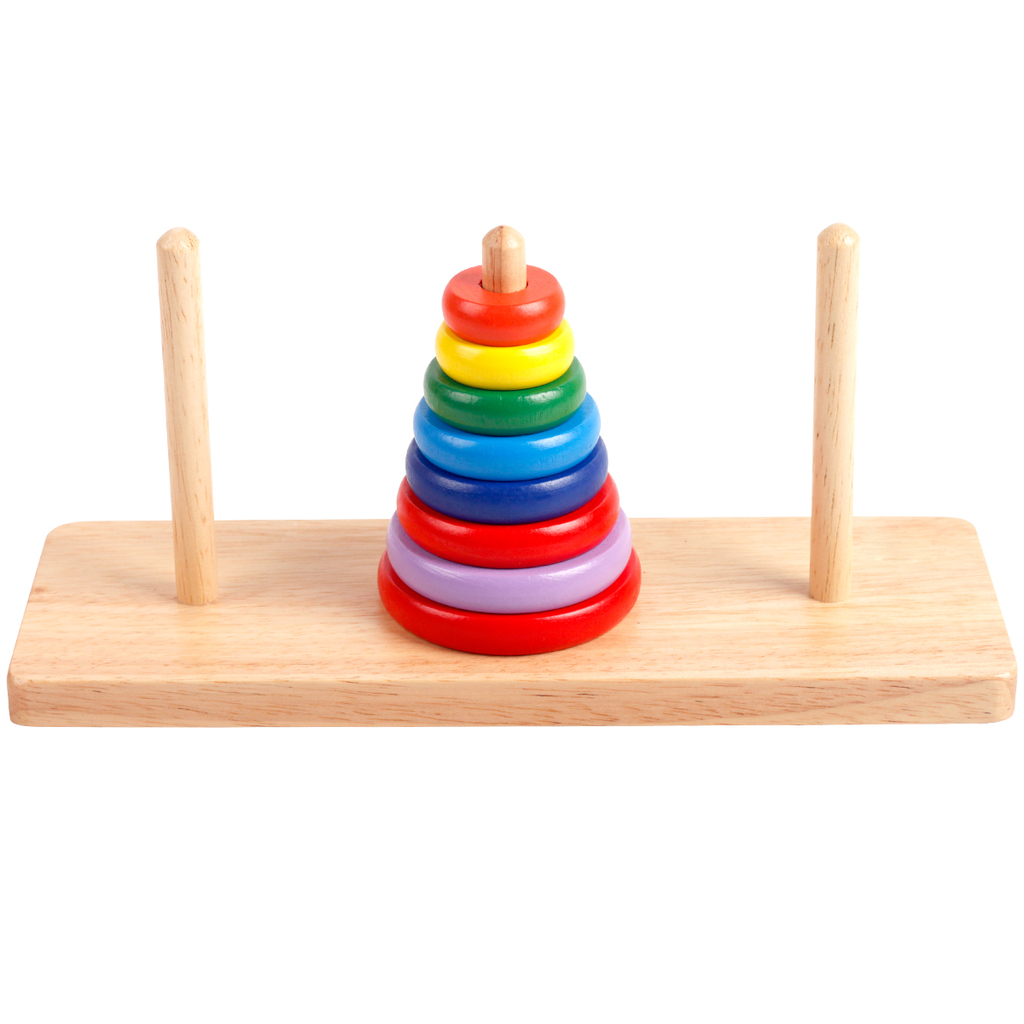
\includegraphics[width=0.6\textwidth]{figure/hanoi.jpg}
  \end{center}

\end{frame}


\begin{frame}[fragile]{Hanoi Tower}
  \begin{python}
def hanoi(a, b, c, n):
    if n==1:
        print("move {0} from {1} to {2}".format(n, a, c))
    else:
        hanoi(a, c, b, n-1)
        print("move {0} from {1} to {2}".format(n, a, c))
        hanoi(b, a, c, n-1)
        
hanoi('a', 'b', 'c', 3)    
  \end{python}
\end{frame}


\begin{frame}[fragile]{求组合$n \choose m$}
  c(n,m)=c(n-1,m-1)+c(n-1,m)
等式左边表示从n个元素中选取m个元素,而等式右边表示这一个过程的另一种实现方法:任意选择n中的某个备选元素为特殊元素,从n中选m个元素可以由此特殊元素的分成两类情况,即m个被选择元素包含了特殊元素和m个被选择元素不包含该特殊元素。
\end{frame}


\subsection{函数式编程}
\begin{frame}[fragile]{函数式编程}
  \begin{easylist}
    & 面向过程的程序设计
    && 把复杂任务分解成简单的任务,简单任务通常以函数表示
    & 函数式编程(Functional Programming)
    && 也可以归结到面向过程的程序设计,但其思想更接近数学计算。
    && 就是越低级的语言,越贴近计算机,抽象程度低,执行效率高,比如C语言;越高级
    的语言,越贴近计算,抽象程度高,执行效率低,比如Lisp语言。
    && 函数式编程就是一种抽象程度很高的编程范式,纯粹的函数式编程语言编写的函数
    没有变量。任意一个函数,只要输入是确定的,输出就是确定的,这种没有副作用的函
    数称为纯函数。
    && 允许把函数本身作为参数传入另一个函数,还允许返回一个函数!
  \end{easylist}
\end{frame}

\begin{frame}[fragile]{高阶函数:Higher-order function}
  \begin{easylist}
    & 变量可以指向函数
    & 函数名也是变量
    & 传入函数
    & 
  \end{easylist}

\end{frame}


\begin{frame}[plain]
  \begin{center}
    \Simley{1}{10}{1}

    \Huge ---END---
  \end{center}
\end{frame}

%%% Local Variables:
%%% mode: latex
%%% TeX-master: "../python"
%%% End:

%\section{模块}

\begin{frame}[fragile]{CH5 模块}
  \begin{enumerate}
     \item 模块介绍
     \item 模块的导入方式
     \item 模块的作用域
     \item 模块的测试
     \item 模块导入的路径搜索
     \item 包
  \end{enumerate}
\end{frame}

\begin{frame}[fragile]{模块介绍}
  \begin{easylist} \easyitem
    & 随着程序代码越写越多,在一个文件里代码就会越来越长,越来越不容易维护。
    & 为了编写可维护的代码,把函数分组放到不同的文件里,这样,每个文件包含的代码
    就相对较少,很多编程语言都采用这种组织代码的方式。
    & 在Python中,一个.py文件就称之为一个模块(Module)。
    && 模块:把多个函数组织到一起,方便其他程序调用
    && 提高了代码的可维护性
    && 编写代码不必从零开始。当一个模块编写完毕,就可以被其他地方引用。

    & 之前我们编写的程序也保存在.py文件中,程序和模块的区别在于:
    && 程序的设计目标是运行
    && 模块的设计目标是由其他程序导入并使用
  \end{easylist}
\end{frame}


\begin{frame}[fragile]{模块的导入方式}
  \begin{easylist}
    & import importable
    & import importable1, importable2, ..., importableN
    & import importable as preferred\_name
    & from importable import *
  \end{easylist}
\end{frame}

\begin{frame}[fragile]{标准库中的模块使用示例}
  \begin{python}
import sys
from pprint import pprint
pprint(sys.path)
  \end{python}

['', \\
 '/usr/lib/python3.4', \\
 '/usr/lib/python3.4/plat-x86\_64-linux-gnu', \\
 '/usr/lib/python3.4/lib-dynload', \\
 '/usr/local/lib/python3.4/dist-packages', \\
 '/usr/lib/python3/dist-packages']

\end{frame}


\begin{frame}[fragile, allowframebreaks]{自定义模块}
  \lstinputlisting[keywordstyle=\ttfamily,
  basicstyle=\rmfamily\normalsize]{src/ch5/hello.py}
  
  \newpage
  ~\\
  \begin{easylist}
    & 行1的注释可以让hello.py文件直接在Unix/Linux/Mac上运行
    & 行2的注释表示.py文件本身使用标准UTF-8编码
    & 第4到6行是一个字符串,表示模块的文档注释,任何模块代码的第一个字符串都被视
    为模块的文档注释
    & 第8行导入了引用的模块
    & 第10行使用\_\_author\_\_变量把作者写进去
  \end{easylist}

\end{frame}


\begin{frame}[fragile]{如何运行}
  \begin{easylist}
    & 方式1:
    && 保存到hello.py文件中
    && 进入命令行,通过cd命令进入hello.py文件所在的目录
    &&& python3 hello.py
    &&& python3 hello.py Tom    
    & 方式2:
    && 启动python交互环境
    &&& \pyinline{import hello}
    &&& \pyinline{hello.sayHi()}
    &&& \pyinline{help(hello)}
    & 观察sys.argv是否包含了模块对应的文件名称
  \end{easylist}

\end{frame}


\begin{frame}[fragile]{模块的作用域}
  \begin{easylist}
    & 在一个模块中,我们可能会定义很多函数和变量,但有的函数和变量我们希望给别人
    使用,有的函数和变量我们希望仅仅在模块内部使用。
    && 通过\_前缀定义的函数和变量只能在模块内部访问
    && 其他函数和变量则是公开可访问的
    && \_\_xxx\_\_ 这样的变量可以被直接引用,但通常有特殊含义
    && 如\_\_name\_\_,  \_\_author\_\_
    & private函数和变量“不应该”被直接引用,而不是“不能”被直接引用,是因为Python
    并没有一种方法可以完全限制访问private函数或变量
  \end{easylist}
\end{frame}


\begin{frame}[fragile, allowframebreaks]{作用域示例: hello2.py}
    \lstinputlisting[keywordstyle=\ttfamily,
  basicstyle=\rmfamily\normalsize]{src/ch5/hello2.py}
 
 \begin{easylist}
    & 请分别用命令行和Python交互环境进行测试
    & 问题:能够在交互环境中通过hello2.\_sayInChinese()访问私有方法?
    & 实验:添加代码,使得程序能够根据命令行传入的参数,决定源代码26行处是调用
  \_sayInChinese()还是\_sayInEnglish()
  && 假设命令行传入的第一个有效参数用于指定语言,中文对应为zh,英文对应为en
  \end{easylist}
  
\end{frame}


\begin{frame}[fragile, allowframebreaks]{hello\_lang.py}
    \lstinputlisting[keywordstyle=\ttfamily,
  basicstyle=\rmfamily\normalsize]{src/ch5/hello_lang.py}
 
 \begin{easylist}
    & python3 hello\_lang.py zh
    & python3 hello\_lang.py en
    & python3 hello\_lang.py zh Tom
    & python3 hello\_lang.py en Tom
  \end{easylist}
\end{frame}


\begin{frame}[fragile]{模块的测试}
  \begin{easylist}
    & 模块本身用于定义函数、类及其他一些内容
    & 在模块中添加一些检查模块本身是否正常工作的测试代码非常有用
    \lstinputlisting[keywordstyle=\ttfamily,
    basicstyle=\rmfamily\normalsize]{src/ch5/hello3.py}   
    & 打开Python交互环境测试
    && \pyinline{import hello3}
    && \pyinline{hello3.hello()}
  \end{easylist}
\end{frame}


\begin{frame}[fragile]{\_\_name\_\_}
  \begin{easylist}
    & \pyinline{hello3.__name__}
    & \pyinline{__name__}
    & 因此,在测试模块时,可以通过如下方式:
    \begin{python}
      if __name__ == '__main__':
          test_suite...
    \end{python}
    && 此时,如果将模块作为独立的程序,条件判断将会满足,继续执行测试代码
    && 如果是import引入模块,则条件表达式不成立,测试代码被忽略
  \end{easylist}
\end{frame}


\begin{frame}[fragile]{如何让Python找到自定义的模块}
  \begin{enumerate}
  \item 在源代码目录下执行python
  \item  设置sys.path
  \end{enumerate}

  \lstinputlisting[keywordstyle=\ttfamily,
    basicstyle=\rmfamily\normalsize]{src/ch5/path_test.py} 
\end{frame}

\subsection{包}
\begin{frame}[fragile]{包的处理}
  \begin{easylist}
    & 包是一个有层次的文件目录结构,由模块和子包组成。
    && 为平坦的名称空间加入了有层次的组织结构
    && 允许程序员把有联系的模块组织到一起
    && 允许分发者使用目录结构而非一大堆文件
    && 有助于解决模块名称冲突问题
  \end{easylist}

\end{frame}


\begin{frame}[fragile]{\_\_init\_\_.py文件}
  \begin{easylist}
    & python的每个模块的包中,都有一个\_\_init\_\_.py文件,有了这个文件,我们才
    能导入这个目录下的module
    && 该文件可以为空
    && 我们在导入一个包时,实际上导入了它的\_\_init\_\_.py文件
  \end{easylist}

\end{frame}

\begin{frame}[fragile]{包的示例}
  graphics/ \\
  ~~~~\_\_init\_\_.py \\
  ~~~~primitive/ \\
  ~~~~~~~~\_\_init\_\_.py \\
  ~~~~~~~~line.py \\
  ~~~~~~~~fill.py \\
  ~~~~~~~~text.py \\
  ~~~~formats/ \\
  ~~~~~~~~\_\_init\_\_.py \\
  ~~~~~~~~png.py \\
  ~~~~~~~~jpg.py \\
\end{frame}

\begin{frame}[fragile]{以上包结构的引用方式}
  \begin{python}
    import graphics.primitive.line
    from graphics.primitive import line
    from graphics.primitive import *
    import graphics.formats.jpg as jpg
  \end{python}
  
  \begin{easylist}
    & 第1行在使用line中的方法时,只能用全名称引用:
    && graphics.primitive.line.xxxx
    & 第2行和第3行的方式,则可以直接使用如下方式
    && line.xxxx, fill.xxxx
    && jpg.xxxx
  \end{easylist}

\end{frame}

\begin{frame}[fragile]{练习}
  \begin{easylist}
    & 实现以上包结构
    && line.py, fill.py 和 text.py中分别写一个draw()方法,在该方法中输入一个简单
    的字符串
    && 在png.py和jpg.py中添加open()方法和close()方法,方法本身只输出一个提示字符
    串即可
  \end{easylist}
\end{frame}


\begin{frame}[fragile]{\_\_init\_\_.py中的\_\_all\_\_}
  \begin{easylist}
    & 通过from p1.p2 import *,可以一次性引入包里面的所有子模块
    & 如果想限定默认引入的子模块集合,可以通过设置\_\_init\_\_.py,例如:
    && 在\_\_init\_\_.py中添加如下内容:\\
    \_\_all\_\_ = ['line', 'fill']
    && from graphics.primitive import *
    && 请完善代码并测试能够直接调用line.xxx()和text.xxxx(),并分析原因
  \end{easylist}
\end{frame}


\begin{frame}[plain]
  \begin{center}
    \Simley{1}{10}{1}

    \Huge ---END---
  \end{center}
\end{frame}

%%% Local Variables:
%%% mode: latex
%%% TeX-master: "../python"
%%% End:

%\section{Python标准库}

\begin{frame}[fragile]{CH6 Python标准库}
  \begin{easylist} \easyitem
    & 内置电池:Battery Included
    && 用于形容Python标准库
    & 标准模块
    && string 
    && io \& sys
    && optparse
    && math
    && random
  \end{easylist}
\end{frame}

\subsection{字符串标准模块:string}
\begin{frame}[fragile]{字符串标准模块:string}
  \begin{easylist}
    & 提供了字符串相关的一些常量 

    \pyinline{string.ascii\_letters} 

    \pyinline{string.ascii\_lowercase} 

    \pyinline{string.ascii\_uppercase} 

    \pyinline{string.digits} 

    \pyinline{string.hexdigits} 

    \pyinline{string.punctuation}

  \end{easylist}
\end{frame}


\subsection{IO输出相关模块}
\begin{frame}[fragile]{IO输出相关标准模块}
  \begin{easylist}
    & 标准输出
    && sys.stdout
    & 字符串输出
    && io.StringIO
    & 以下输出方式是等价的
  \end{easylist}

  \begin{python}
    import sys,io
    print("hello")
    print("hello", file=sys.stdout)
    sys.stdout.write("hello\n") #python3 中会同时输出字符串的数量
  \end{python}
\end{frame}

\begin{frame}[fragile]{StringIO}
  \begin{easylist}
    & 如果要把输出重定向到字符串中,在需要时再获取,可以StringIO
    && 注意:Python 2.x和3.x在输出时的行为不同
  \end{easylist}

  \begin{python}
    import sys, io
    out = io.StringIO()
    sys.stdout = out
    out.write('how are you')
    print('hello')
    print('guys')
    sys.stdout = sys.__stdout__
    print(out.getvalue())
  \end{python}
\end{frame}


\subsection{命令行参数模块}
\begin{frame}[fragile, allowframebreaks]{命令行参数模块:optparse}
  \begin{easylist}
    & 如何指定脚本运行的命令行参数
    && 例如,Linux命令 ls --l
    && Python提供的optparse模块对命令行参数的解析处理提供了良好的支持
  \end{easylist}

  \lstinputlisting[keywordstyle=\ttfamily]{src/ch6/cmdopt.py}
\end{frame}


\begin{frame}[fragile]{分析}
  \begin{easylist}
    & 说明
    && 长短参数名称
    && 参数对应的变量名称及获取方式
    && metavar参数:提醒用户该命令行参数所期待的参数,参数中的字符串会自动变为大写
    && parser.parse\_args()
    &&& 解析后得到的options拥有两个属性:filename和verbose

    & 假设文件保存到cmdopt.py,执行:
    && python3 cmdopt.py -f cmdopt.py,观察输出结果
    && python3 cmdopt.py -h
  \end{easylist}

\end{frame}


\subsection{数学标准模块:math}
\begin{frame}[fragile]{数学标准模块:math}
  \begin{easylist}
    & math.exp(x)
    \[e^x\]
    & math.sqrt(x)
    \[\sqrt{x}\]
    & math.pi
    & math.e
    & math.log
    && \pyinline{math.log(math.e)}
    && \pyinline{math.log2(2)}
    && \pyinline{math.log10(10)}
    && \pyinline{math.log1p(math.e - 1)}
  \end{easylist}
\end{frame}


\subsection{随机数模块:random}
\begin{frame}[fragile]{随机数标准模块:random}
  \begin{easylist}
    & 生成$[0, 1)$之间的随机数
    && \pyinline{import random}
    && \pyinline{random.random()}
    & random.gauss(mu, sigma)生成一个均值为mu,标准值为sigma的符合高斯分布的随机
    数
    && \pyinline{random.gauss(0, 1)}
  \end{easylist}
\end{frame}

\begin{frame}[fragile]{高斯分布模拟}
  \begin{easylist}
    & 通过random.gauss()生成一组随机数
    & 通过柱状图显示结果
  \end{easylist}
  \pause
  \begin{python}
    import matplotlib.pyplot as plt
    import random

    data = [random.gauss(0,1) for x in range(10000)]
    plt.hist(data, bins = 50)
    plt.show()
  \end{python}
\end{frame}

\begin{frame}[fragile]{Result}
  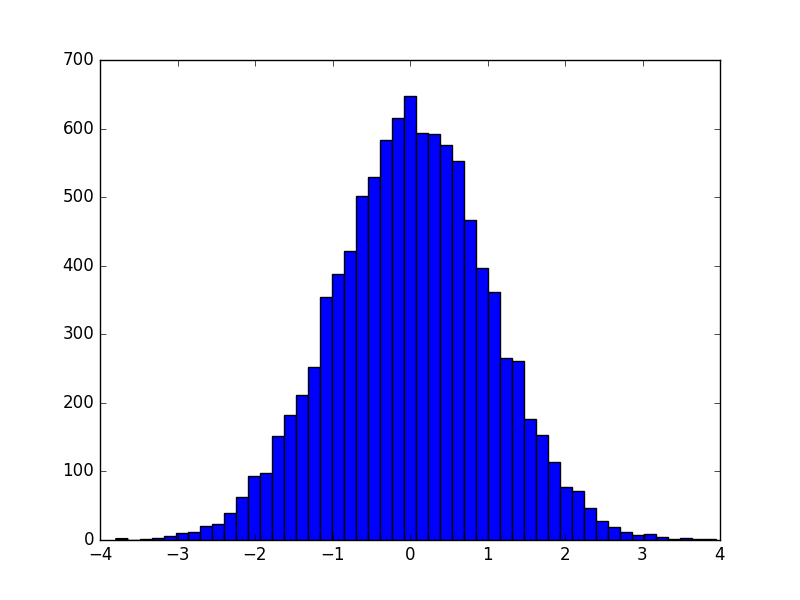
\includegraphics[width=0.8\textwidth]{figure/gauss1.png}
\end{frame}


\begin{frame}[fragile]{高斯分布模拟}
  \begin{easylist}
    & 通过高斯分布的概率密度函数生成(x, y)对,利用散点图显示结果
    \[ f(x) = \dfrac{1}{\sigma \sqrt{2 \pi}} e^{-\dfrac{(x-\mu)^2}{2 \sigma^2}} \]
  \end{easylist}
\end{frame}

\begin{frame}[fragile]{高斯分布模拟代码}
  \lstinputlisting[keywordstyle=\ttfamily]{src/ch6/gauss.py}
\end{frame}

\begin{frame}[fragile]{Result}
  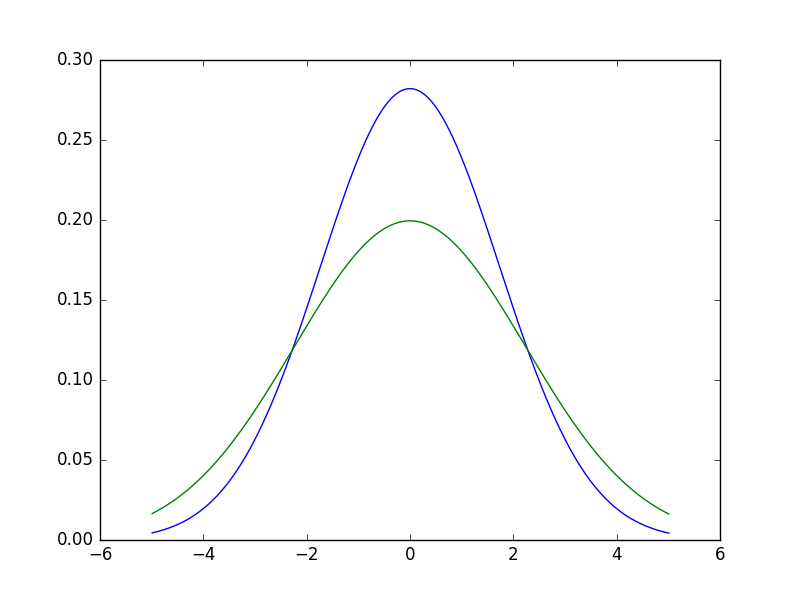
\includegraphics[width=0.8\textwidth]{figure/gauss2.png}
\end{frame}


\subsection{日志处理模块: logging}
\begin{frame}[fragile]{日志处理标准库:logging}
  \begin{easylist}
    & 日志的作用
    
    & 日志的级别
    && DEBUG:详细的信息,通常只出现在诊断问题上
    && INFO:确认一切按预期运行
    && WARNING:一个迹象表明,一些意想不到的事情发生了,或表明一些问题在不久的将来(例如。磁盘空间低”)。这个软件还能按预期工作。
    && ERROR:个更严重的问题,软件没能执行一些功能
    && CRITICAL:一个严重的错误,这表明程序本身可能无法继续运行
    
    & 优先级关系
    && CRITICAL > ERROR > WARNING > INFO > DEBUG
  \end{easylist}
\end{frame}


\begin{frame}[fragile]{日志示例}
  
  \begin{python}
import logging

logging.debug('debug message')
logging.info('info message')
logging.warning('warning message')
logging.error('error message')
logging.critical('critical message')
  \end{python}

\begin{easylist}
  & 默认输出到控制台,级别在warning及以上的信息会输出,
  & 可以通过basicConfig设置输出方式和记录级别
\end{easylist}
\end{frame}

\begin{frame}[fragile]{日志示例:输出到文件}
  \begin{python}
import os
import logging


FILE = os.getcwd()
logging.basicConfig(filename=os.path.join(FILE, 'log.txt'),
                    level=logging.DEBUG)
logging.debug('some debug messages...')
logging.info('some info messages...')
logging.warning('some warning messages...')
  \end{python}
\end{frame}


% \subsection{正则表达式模块:re}
% \begin{frame}[fragile]{正则表达模块:re}
%   ~
% \end{frame}


% \subsection{os与os.path标准模块}
% \begin{frame}[fragile]{os与os.path标准模块}
%   ~
% \end{frame}

\begin{frame}[fragile]{第3方扩展:Requests}
  \begin{easylist}
    & 通过Requests包可以更方便地实现Web数据的采集
    && Install: pip install requests
  \end{easylist}

  \begin{python}
import requests

url = 'http://download.pchome.net/wallpaper/zhiwu/'
response = requests.get(url)
print(response.text)    
  \end{python}
\end{frame}

\begin{frame}[fragile]{BeautifulSoup}
  \begin{easylist}
    & 怎么解析抓取到的网页,例如,如何抽取网页中的图片?
    & BeautifulSoup --- Html Parser
    && Install: pip install beautifulsoup4
  \end{easylist}
\end{frame}

\begin{frame}[fragile]{Example}
  \begin{python}
import requests

url = 'http://download.pchome.net/wallpaper/zhiwu/'
response = requests.get(url)
print(response.text)

from bs4 import BeautifulSoup as soup
doc = soup(response.text, 'html')
images = [element.get('src') for element in doc.find_all('img')]    
  \end{python}
\end{frame}

\begin{frame}[fragile]{课堂练习}
  \begin{easylist}
    & 编写程序,实现对任意指定网页,下载该网页包含的所有图片到指定的文件夹当中
  \end{easylist}

\end{frame}

\begin{frame}[fragile]{Thanks}
  ~
\end{frame}

%%% Local Variables:
%%% mode: latex
%%% TeX-master: "../python"
%%% End:

%\section{CH7 面向对象编程}

\begin{frame}[fragile]{CH7 面向对象编程}
  \begin{easylist} \easyitem
    & 简介
    & 类和实例
    & 数据封装
    & 继承和多态
    & Duck Typing
    & 获取对象信息
    & 实例属性和类属性
    & 高级特性
    & 小结
  \end{easylist}
\end{frame}

\subsection{简介}
\begin{frame}[fragile]{\newsec 面向对象编程简介}
  \begin{easylist}
    & 面向对象编程OOP(Object Oriented Programming)
    && 一种程序设计思想,OOP把对象作为程序的基本单元,一个对象包含了数据和操作
    数据的函数。
    && 面向过程的程序设计把计算机程序视为一系列的命令集合,即一组函数的顺序执
    行
    && OOP通过把大块函数切割为小块函数来降低系统的复杂度
    && OOP把计算机程序看做是一组对象的集合,程序执行就是一些列消息在各个对象之
    间传递,给对象发消息实际上就是调用对象对应的关联函数
    & OOP特点
    && 封装、继承、多态
    & 类(Class)与实例(Instance)
  \end{easylist}
\end{frame}

\begin{frame}[fragile]{举例: 面向过程方式}
  处理学生成绩并打印输出,面向过程设计方式:

  \begin{python}
std1 = {'name': '韩寒', 'score':85}    
std2 = {'name': '黄锤', 'score':90}

def print_score(std):
    print('%s: %s' % (std['name'], std['score']))

print_score(std1)
print_score(std2)
  \end{python}
\end{frame}

\begin{frame}[fragile]{举例: 面向对象方式}
  \begin{python}
class Student(object):
    def __init__(self, name, score):
        self.name = name
        self.score = score

    def print_score(self):
        print('%s: %s' % (self.name, self.score))

if __name__ == '__main__':
    han = Student('韩寒', 85)
    huang = Student('黄锤', 90)
    han.print_score()
    huang.print_score()
  \end{python}
\end{frame}


\begin{frame}[fragile]{例子解释}
  \begin{easylist}
    & class关键字
    & object
    & self
  \end{easylist}
\end{frame}


\subsection{类和实例}
\begin{frame}[fragile]{\newsec 类和实例}
  \begin{easylist}
    & 类是抽象的模板,比如Student类
    & 实例是根据类创建出来的一个个具体的“对象”
    & 每个对象都拥有相同的方法,但各自的数据可能不同。
  \end{easylist}
\end{frame}

\begin{frame}[fragile]{类的定义}
  通过class关键字定义类

  \begin{python}
class Student(object):
    pass
  \end{python}

  \begin{easylist}
    & class后面紧接着是类名
    & 类名通常是大写开头的单词
    & 类名后紧接着是(object),表示该类是从哪个类继承下来的
    && object是所有类最终都会继承的类
  \end{easylist}
\end{frame}


\begin{frame}[fragile]{类的实例化}
  类名+()实现, 例如:

  \begin{python}
    xiaoming = Student('小明', 85)
    print(xiaoming)    
    print(Student)
  \end{python}

  <\_\_main\_\_.Student object at 0x7f16e99ee710> \\
  <class '\_\_main\_\_.Student'>
\end{frame}

\begin{frame}[fragile]{实例的变量绑定}
  可以自由地给一个实例变量绑定属性和方法,比如,给实例xiaoming绑定一个name属性,
  和speak()方法:

\begin{python}
def speak(something):
    print('speak:' , something)

xiaoming.name = 'xiaoming'
xiaoming.speak = speak
print(xiaoming.name)
xiaoming.speak('hello')
\end{python}
\end{frame}


\begin{frame}[fragile]{实例的初始化}
  通过定义特殊的\_\_init\_\_方法,在创建实例的时候,可以绑定期望的属性

\begin{python}
  class Student(object):

    def __init__(self, name, score):
        self.name = name
        self.score = score
\end{python}

\begin{easylist}
  & \_\_init\_\_方法的第一个参数永远是self,表示创建的实例本身
  & 在\_\_init\_\_方法内部,可以把各种属性绑定到self,因为self就指向创建的实例本
  身。

\end{easylist}

\end{frame}


\begin{frame}[fragile]{\_\_init\_\_()解释}
  \begin{easylist}
    & 有了\_\_init\_\_方法,在创建实例的时候,就不能传入空的参数了,必须传入与该
    方法匹配的参数,但self不需要传,Python解释器自己会把实例变量传进去
  
    \pyinline{xiaoli = Student('小李', 80)}
    & 和普通的函数相比,在类中定义的函数只有一点不同,就是第一个参数永远是实例变
    量self,并且,调用时,不用传递该参数。除此之外,类的方法和普通函数没有什么区
    别,所以,仍然可以用默认参数、可变参数、关键字参数和命名关键字参数。

  \end{easylist}
\end{frame}

\subsection{数据封装}
\begin{frame}[fragile]{\newsec 数据封装}
  \begin{easylist}
    & 实例中拥有的属性、方法,被封装到实例中
    & 在实例中使用本身的属性或方法,用self.xxx方式
    & 在类中定义方法时,第一个参数必须为self
    & 在外部调用方法时,无需指定self,类会自动把self传入
    & 封装的优点是调用简单,无需关心内部实现细节
  \end{easylist}
\end{frame}


\subsection{继承和多态}
\begin{frame}[fragile]{\newsec 继承和多态}
  \begin{block}{}
    在OOP程序设计中定义一个class的时候,可以从某个现有的class继承,新的class称为
    子类(Subclass),而被继承的class称为基类、父类或超类(Base class、Super
    class)。
  \end{block}

  \begin{python}
    class Postgraduate(Student):
        '''post graduate student'''
        pass
  \end{python}

  \color{blue}继承可以把父类的所有功能都直接拿过来,这样就不必从零做起,子类只需要新增自己特
  有的方法,也可以把父类不适合的方法覆盖重写(多态)。

\end{frame}


\begin{frame}[fragile]{多态}
  \begin{easylist}
    & 多态即多种状态
    & 同一个实体同时具有多种形式, 对基类的引用指向子类的对象
    && 例子中,子类和父类都存在相同的sayHi()方法,此时,子类的sayHi()覆盖了父类的
    sayHi(),在代码运行的时候,总是会调用子类的sayHi()
  \end{easylist}
\end{frame}


\begin{frame}[fragile, allowframebreaks]{多态示例}
  \lstinputlisting[keywordstyle=\ttfamily]{src/ch7/student.py}
\end{frame}


\begin{frame}[fragile]{isinstance}
  \begin{easylist}
    & 可以用isinstance判断实例的类型
  \end{easylist}

\begin{python}
  wang = Postgraduate('王二小', 80)
  isinstance(wang, Postgraduate) #True or False?
  isinstance(wang, Student) #True or False?
\end{python}
\end{frame}


\subsection{Duck Typing}
\begin{frame}[fragile]{\newsec Duck Typing\footnote{\url{https://en.wikipedia.org/wiki/Duck\_typing}}}
  \begin{easylist}
    & 对于静态语言(如Java),如果需要传入Student类型,则传入的对象必须是Student类
    型或者它的子类  
    & 对于Python这样的动态语言,只需要保证传入的对象有sayHi()方法就可以
    & 这种设计方法称之为鸭子类型:
    && \color{blue} 一个对象有效的语义,不是由继承自特定的类或实现特定的接口,而是由当前方法
    和属性的集合决定。
  \end{easylist}

\begin{python}
class Robot():
    def sayHi(self):
        print("I'm robot")
        
meet(Robot())    
\end{python}
\end{frame}

\begin{frame}[fragile]{Duck Typing}
  \begin{block}{Duck Test}
    {\huge "} When I see a bird that walks like a duck and swims like a duck and quacks
    like a duck, I call that bird a duck.{\huge "}

    \begin{flushright}
      \scriptsize{--- Indiana poet James Whitcomb Riley (1849--–1916)}
    \end{flushright}
  \end{block}
\end{frame}

\begin{frame}[fragile, allowframebreaks]{Duck Typing示例}
  \lstinputlisting{src/ch7/duck.py}
\end{frame}


\subsection{获取对象信息}
\begin{frame}[fragile]{\newsec 获取对象信息}
  \begin{easylist}
    & 当我们拿到一个对象的引用时,如何知道这个对象是什么类型、有哪些方法呢?
    && isinstance(): 判断对象是否为某个类的实例 
    && type(): 判断对象的类型
    && dir(): 获得对象的所有属性和方法
  \end{easylist}
\end{frame}

\begin{frame}[fragile]{type()}
  \begin{python}
    type(123) == type(456) 
    type(123) == int 
    type('hello') == str 

    import types
    type(abs) == types.BuiltinFunctionType
    type(lambda x:x) == types.LambdaType
    type((x for x in range(10)))==types.GeneratorType

    def hi():
        pass
    type(hi) == types.FunctionType
  \end{python}
\end{frame}

\begin{frame}[fragile]{dir()}
  \begin{easylist}
    & 获得一个对象的所有属性和方法,可以使用dir()函数,它返回一个包含字符串的list
  \end{easylist}

  \begin{python}
    wang = Postgraduate('王小二', 80)
    dir(wang)

    ['__class__', '__delattr__', '__dict__', '__dir__', '__doc__', '__eq__', '__format__', '__ge__', '__getattribute__', '__gt__', '__hash__', '__init__', '__le__', '__lt__', '__module__', '__ne__', '__new__', '__reduce__', '__reduce_ex__', '__repr__', '__setattr__', '__sizeof__', '__str__', '__subclasshook__', '__weakref__', 'name', 'print_score', 'sayHi', 'score']
  \end{python}
\end{frame}


\subsection{实例属性和类属性}
\begin{frame}[fragile]{\newsec 实例属性和类属性}
  \begin{easylist}
    & 实例属性隶属于实例
    && 通过self或实例绑定属性
    & 类属性隶属于类,其所有实例均可以访问到
    && 直接在class中定义的属性
  \end{easylist}
\end{frame}

\begin{frame}[fragile, allowframebreaks]{实例属性和类属性示例}
  \begin{python}
#实例属性示例
class Student(object):
    def __init__(self, name):
        self.name = name #通过self绑定属性
        
s = Student('Bob')
s.score = 90 #通过实例绑定属性
print("%s : %s" % (s.name,  s.score))
\end{python}

\newpage

\begin{python}
#类属性示例
class Student(object):
    name = 'Student'
\end{python}

  $>>>$ s = Student() \# 创建实例s \\
  $>>>$ print(s.name) \# 打印name属性,因为实例并没有name属性,所以会继续查找class的
  name属性 \\
  Student \\
  $>>>$ print(Student.name) \# 打印类的name属性 \\
  Student \\
  $>>>$ s.name = 'Michael' \# 给实例绑定name属性 \\

  \newpage

  $>>>$ print(s.name) \# 由于实例属性优先级比类属性高,因此,它会屏蔽掉类的name属性 \\
  Michael \\
  $>>>$ print(Student.name) \# 但是类属性并未消失,用Student.name仍然可以访问 \\
  Student \\
  $>>>$ del s.name \# 如果删除实例的name属性 \\
  $>>>$ print(s.name) \# 再次调用s.name,由于实例的name属性没有找到,类的name属性就显
  示出来了 \\
  Student    
\end{frame}


\subsection{小结}
\begin{frame}[fragile]{\newsec 面向对象编程小结}
  \begin{easylist}
    & 类是创建实例的模板,而实例则是一个一个具体的对象,各个实例拥有的数据都互相独立,互不影响;

    & 方法就是与实例绑定的函数,和普通函数不同,方法可以直接访问实例的数据;
    & 通过在实例上调用方法,我们就直接操作了对象内部的数据,但无需知道方法内部的实现细节。
    & 和静态语言不同,Python允许对实例变量绑定任何数据
    && 也就是说,对于两个实例变量,虽然它们都是同一个类的不同实例,但拥有的变量
    名称都可能不同
    & Duck Typing
    & 实例属性与类属性
  \end{easylist}
\end{frame}

\begin{frame}[fragile]{练习}
  \begin{easylist}
    & 假设磁盘中存在一个学生成绩的文本文件,每行格式如下:
    && 123,成工,高等数学,80
    && 123,成工,线性代数,85
    && 124,王小二,线性代数,80
    && $\cdots$
    & 利用OOP设计思想,实现以下功能:
    && 按照学号或姓名查找满足条件的学生的所有成绩信息,并输出其平均分
    && 根据课程名称输出所有学生的成绩,并输出平均成绩、最高分和最低分
  \end{easylist}

\end{frame}


\begin{frame}[fragile, allowframebreaks]{Test}
  \begin{python}
class Query():
    def __init__(self, filename):
        slef.filename = filename
        
    def _parse_line(self, line):
        return 123, 'zhang', 'math', 80
        
    def find_by_number(self, num):
        scores = {}
        f = open(self.filename, 'r')
        for line in f:
            n, name, course, score = self._parse_line(line)
            if n == num:
                scores[course] = score
                
        total = 0
        for course, score in scores.items():
            print(course, '==>', score)
            total += score
        print('avg', total/len(scores))    

    if __name__ == '__main__':
        q = Query('some_file.txt')
        q.find_by_number(123)
  \end{python}
\end{frame}



\subsection{Python面向对象的高级特性}
\begin{frame}[fragile]{Python面向对象的高级特性}
  \begin{easylist}
    & \_\_slots\_\_
    & @property
    & 多重继承
    & 定制类
    & 枚举类
    & 元类
  \end{easylist}
\end{frame}


\subsubsection{\_\_slots\_\_}
\begin{frame}[fragile, allowframebreaks]{\_\_slots\_\_的引入}
  实例绑定与类的绑定示例
  \begin{python}
class Student(object):
    pass

s = Student()
s.name = 'Lucy'
print(s.name) # 输出Lucy

def set_age(self, age):
    self.age = age

from types import MethodType
s.set_age = MethodType(set_age, s) # 给实例绑定方法
s.set_age(25) # 调用实例方法
print(s.age) # 测试结果

s2 = Student() # 创建新的实例
s2.set_age(25) # 尝试调用方法
  \end{python}

  调用s2.set\_age(25)会给出错误提示:对象Student没有属性set\_age,此时,为了给所有
  实例都绑定方法,可以给class绑定方法,如下:
\begin{python}
def set_score(self, score):
    self.score = score

Student.set_score = set_score # 在类级别上绑定方法

s.set_score(100)
print(s.score)
s2.set_score(99)
print(s2.score)
\end{python}

\begin{easylist}
  & 新问题:
  && 如果要限制对实例的属性随意赋值,该怎么处理?
  && \_\_slots\_\_
\end{easylist}
\end{frame}



\begin{frame}[fragile]{\_\_slots\_\_}
  \_\_slots\_\_规定了class能添加的属性

\begin{python}
class Student(object):
    __slots__ = ('name', 'age')

s = Student()
s.age = 25
s.score = 90 # Error!
\end{python}

AttributeError: 'Student' object has no attribute 'score'

注意:\_\_slots\_\_定义的属性仅对当前类实例起作用,对继承的子类是不起作用的
\end{frame}


\subsubsection{@property}
\begin{frame}[fragile, allowframebreaks]{@property的引入}
  \begin{easylist}
    & 在绑定属性时,如果我们直接把属性暴露出去,虽然写起来很简单,但是,没办法检
    查参数
    && 例如,成绩score,我们希望把成绩的范围限制到0--100之间
    && 思路:增加get\_score()和set\_score()对进行读取和修改
  \end{easylist}

  \begin{python}
class Student(object):
    def get_score(self):
        return self._score

    def set_score(self, value):
        if not isinstance(value, int):
            raise ValueError('score必须是整数!')    
        if value < 0 or value > 100:
            raise ValueError('score必须是一个0到100之间的数字')
        self._score = value
  \end{python}

  \newpage
  \begin{python}
s = Student()
s.set_score(60)
print(s.get_score())
s.set_score(999) # Error!
  \end{python}

  \begin{easylist}
    & 上面的调用方法又略显复杂
    & 能否仍然使用s.score = 某个数字, 同时还能判断赋予的数值是否满足要求?
    & Python的@property装饰器负责把一个方法变成属性调用
  \end{easylist}
\end{frame}

\begin{frame}[fragile, allowframebreaks]{@property示例}
  \begin{python}
class Student(object):
    |\color{red}@property|
    def score(self):
        return self._score

    |\color{red}@score.setter|
    def score(self, value):
        if not isinstance(value, int):
            raise ValueError('score必须是整数!')    
        if value < 0 or value > 100:
            raise ValueError('score必须是一个0到100之间的数字')
        self._score = value   
\end{python}

\newpage
\begin{python}
s = Student()
s.score = 60
print(s.score)
|\color{red}s.score = 999| # Error!
\end{python}
\end{frame}

\subsubsection{多重继承}
\begin{frame}[fragile]{多重继承}
  \begin{easylist}
    & 继承是面向对象编程的一个重要的方式,因为通过继承,子类就可以扩展父类的功能。
    & 假设我们要实现以下4种动物:
    && Dog - 狗
    && Bat - 蝙蝠
    && Parrot - 鹦鹉
    && Ostrich - 鸵鸟
  \end{easylist}

\end{frame}

\begin{frame}[fragile]{设计思路}
  \begin{columns}
    \begin{column}{.5\textwidth}
      按照哺乳动物和鸟类归类:


    \end{column}
    
    \begin{column}{.5\textwidth}
      按照“能跑”和“能飞”来归类
      
    \end{column}
  \end{columns}
\end{frame}

\begin{frame}[fragile]{设计思路}
  \begin{python}
class Animal(object):
    pass

# 大类:
class Mammal(Animal):
    pass

class Bird(Animal):
    pass

# 各种动物:
class Dog(Mammal):
    pass

class Bat(Mammal):
    pass

class Parrot(Bird):
    pass

class Ostrich(Bird):
    pass    
  \end{python}
\end{frame}


\begin{frame}[fragile]{定义Runnable和Flyable}
  \begin{python}
class Runnable(object):
    def run(self):
        print('Running...')

class Flyable(object):
    def fly(self):
        print('Flying...')
  \end{python}
\end{frame}

\begin{frame}[fragile]{多重继承示例}
  \begin{python}
class Dog(Mammal, Runnable):
    pass

class Bat(Mammal, Flyable):
    pass    
  \end{python}

  \begin{easylist}
    & 通过多重继承,一个子类就可以同时获得多个父类的所有功能。
  \end{easylist}
\end{frame}

\begin{frame}[fragile]{MixIn}
  \begin{easylist}
    & 在设计类的继承关系时,通常,主线都是单一继承下来的
    && 如:Ostrich继承自Bird
    & 如果需要“混入”额外的功能,通过多重继承就可以实现
    && 比如,让Ostrich除了继承自Bird外,再同时继承Runnable
    & 这种设计方法通常称之为MixIn
    && 为了更好地看出继承关系,通常采用MixIn作为功能性的父类名称的后缀
  \end{easylist}
\end{frame}

\begin{frame}[fragile]{MixIn实例}
  \begin{python}
class RunnableMixIn(object):
    def run(self):
        print('Running...')

class FlyableMixIn(object):
    def fly(self):
        print('Flying...')

class Dog(Mammal, RunnableMixIn):
    pass    
  \end{python}
\end{frame}

\subsubsection{对类进行定制}
\begin{frame}[fragile]{对类进行定制}
  \begin{easylist}
    & \_\_len\_\_
    & \_\_str\_\_
    & \_\_repr\_\_
    & \_\_iter\_\_ 与 \_\_next\_\_
    & \_\_getitem\_\_
    & \_\_getattr\_\_
    & \_\_call\_\_
  \end{easylist}
\end{frame}

\begin{frame}[fragile]{\_\_len\_\_}
  \begin{python}
    class Panda(object):
    def __init__(self):
        pass

    def __len__(self):
        return 10

panda = Panda()
len(panda)
  \end{python}
\end{frame}

\begin{frame}[fragile]{\_\_str\_\_与\_\_repr\_\_}
  \begin{python}
class Panda(object):
    def __init__(self):
        pass

    def __str__(self):
        return '熊猫'

panda = Panda()
print(panda) # 熊猫
panda    # <__main__.Panda at 0x7f20e414db38>
  \end{python}
  
  \begin{easylist}
    & 如何解决非print时输出地址的问题?
  \end{easylist}
\end{frame}


\begin{frame}[fragile]{\_\_str\_\_与\_\_repr\_\_}
  \begin{python}
class Panda(object):
    def __init__(self):
        pass

    def __str__(self):
        return '熊猫'

    __repr__ = __str__
panda = Panda()
print(panda) # 熊猫
panda    # 熊猫
  \end{python}  
\end{frame}


\begin{frame}[fragile]{\_\_iter\_\_ 与 \_\_next\_\_}
  \begin{easylist}
    & 方便通过for循环对对象维持的数据进行遍历
    && 例如:假设拥有一个斐波那契数列的类Fib,通过以下语句循环输出:
    \begin{python}
for n in Fib(10):
     print(n)
    \end{python}
    && 我们希望输出1, 1, 2, 3, 5, 8, 13, 21, 34, 55
    && 怎么实现Fib? 
  \end{easylist}
\end{frame}

\begin{frame}[fragile, allowframebreaks]{Fib}
  \lstinputlisting{src/ch7/fib.py}
\end{frame}

\begin{frame}[fragile]{扩展练习}
  \begin{easylist}
    & 用Python编写程序,对本机指定目录下的文件进行扫描,把所有指定后缀名的文档
    名称统一输出到一个文本文件中。
  \end{easylist}
\end{frame}


\begin{frame}[fragile]{END}
  ~
\end{frame}

%%% Local Variables:
%%% mode: latex
%%% TeX-master: "../python"
%%% End:

\section{CH8 异常、调试与测试}

\begin{frame}[fragile]{CH8 异常、调试与测试}
  \begin{easylist} \easyitem
    & 异常
    && Python的异常处理使用方法
    && Python的异常继承关系
    && 利用raise抛出异常
    & 调试
    && print调试法
    && logging调试法
    && assert
    && pdb
    & 单元测试
  \end{easylist}
\end{frame}

\subsection{异常处理}
\subsubsection{异常处理使用方法}
\begin{frame}[fragile]{异常处理}
  \begin{easylist}
    & 程序在编写过程中,有大量情况需要考虑
    && 除数是否为0
    && 打开文件时,需要判断文件是否存在,有无权限
    && ...
    & 异常可以简化这一处理过程
    & Python的错误处理机制
    && try...except...finally...
  \end{easylist}
\end{frame}

\begin{frame}[fragile]{try}
  \begin{python}
try:
    print('try...')
    r = 10 / 0
    print('result:', r)
except ZeroDivisionError as e:
    print('except:', e)
finally:
    print('finally...')
print('END')    
  \end{python}

  try... \\
  except: division by zero \\
  finally... \\
  END \\
\end{frame}

\begin{frame}[fragile]{try}
  \begin{python}
try:
    print('try...')
    r = 10 / 2
    print('result:', r)
except ZeroDivisionError as e:
    print('except:', e)
finally:
    print('finally...')
print('END')    
  \end{python}

  try... \\
  result: 5.0 \\
  finally... \\
  END \\  
\end{frame}

\begin{frame}[fragile]{Python异常处理的规则}
  \begin{easylist}
    & 遇到第一个满足条件的异常,执行该异常下的语句,忽略后续的其它异常
    & finally永远会被执行
  \end{easylist}

\end{frame}

\subsubsection{异常继承关系}
\begin{frame}[fragile]{Python异常的继承关系}
  \begin{easylist}
    & Python的错误也是class,都继承自BaseException
    && 在使用except时需要注意的是,它不但捕获该类型的错误,还把其子类也“一网打尽”。
  \end{easylist}

  \begin{python}
lst = [x for x in range(10)]
try:
    n = lst[15]
except LookupError as e:
    print('LookupError ', e)
except IndexError as e:
    print('IndexError ', e)
  \end{python}
\end{frame}


\begin{frame}[fragile]{Python异常继承关系示例}
  \begin{center}
    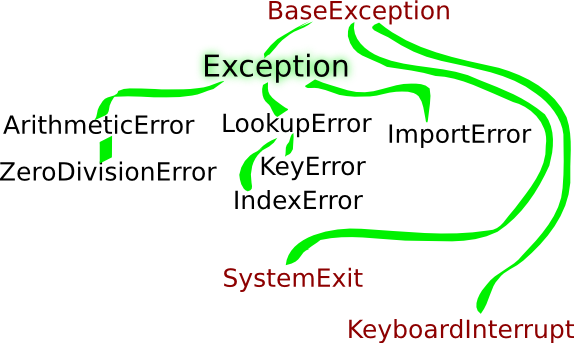
\includegraphics[width=0.8\textwidth]{figure/exception-hierarchy.png}
  \end{center}
  \url{https://docs.python.org/3/library/exceptions.html#exception-hierarchy}
\end{frame}

\subsubsection{利用raise抛出异常}
\begin{frame}[fragile]{抛出异常}
  \begin{easylist}
    & 可以用raise语句来引发一个异常。异常/错误对象必须有一个名字,且它们应是Error或Exception类的子类。
  \end{easylist}

\end{frame}


\begin{frame}[fragile, allowframebreaks]{raise示例}
  \begin{python}
class Student(object):
    |\color{red}@property|
    def score(self):
        return self._score

    |\color{red}@score.setter|
    def score(self, value):
        if not isinstance(value, int):
            raise ValueError('score必须是整数!')    
        if value < 0 or value > 100:
            raise ValueException('score必须在0到100之间')
        self._score = value   
\end{python}

\newpage
\begin{python}
s = Student()
s.score = 60
print(s.score)
|\color{red}s.score = 999| # Error!
\end{python}
\end{frame}


\begin{frame}[fragile, allowframebreaks]{异常可以自定义}
  \begin{easylist}
    & 例如:把以上的score判断条件不满足时,抛出的异常更改为自定义异常
  \end{easylist}

  \begin{python}
class ScoreException(Exception):
    def __init__(self, msg):
        self.msg = msg
        
    def __str__(self):
        return 'ScoreException: ' + repr(self.msg)
    
class Student(object):
    @property
    def score(self):
        return self._score

    @score.setter
    def score(self, value):
        if not isinstance(value, int):
            raise ScoreException('score必须是整数!')    
        if value < 0 or value > 100:
            raise ScoreException('score必须在0到100之间')
        self._score = value   
        
try:       
    s = Student()
    s.score = 60
    print(s.score)
    s.score = 999
except ScoreException as e:
    print(e)    
  \end{python}
\end{frame}

\begin{frame}[fragile]{异常总结}
  \begin{easylist}
    & Python内置的try...except...finally用来处理错误十分方便
    && 出错时,会分析错误信息并定位错误发生的代码位置更为关键
    & 程序也可以主动抛出错误,让调用者来处理相应的错误
    && 应在文档中写清楚可能会抛出哪些错误,以及错误产生的原因
  \end{easylist}
\end{frame}


\subsection{调试}
\begin{frame}[fragile]{调试}
  \large Bug and Debug
  \begin{columns}[onlytextwidth,T]
    \begin{column}{0.5\textwidth}
      \begin{block}{\small 格蕾丝·赫柏(Grace Murray Hopper)}
        \scriptsize{赫柏是一位为美国海军工作的电脑专家。1945年的一天,赫柏
        对Harvard Mark II设置好17000个继电器进行编程后,技术人员在进行整机运行时,
        它突然停止了工作。于是他们爬上去找原因,发现这台巨大的计算机内部一组继电
        器的触点之间有一只飞蛾,这显然是由于飞蛾受光和热的吸引,飞到了触点上,然
        后被高电压击死。所以在报告中,赫柏用胶条贴上飞蛾,并把“bug”来表示"一个在
        电脑程序里的错误"。}
      \end{block}
    \end{column}
    \begin{column}{0.45\textwidth}
      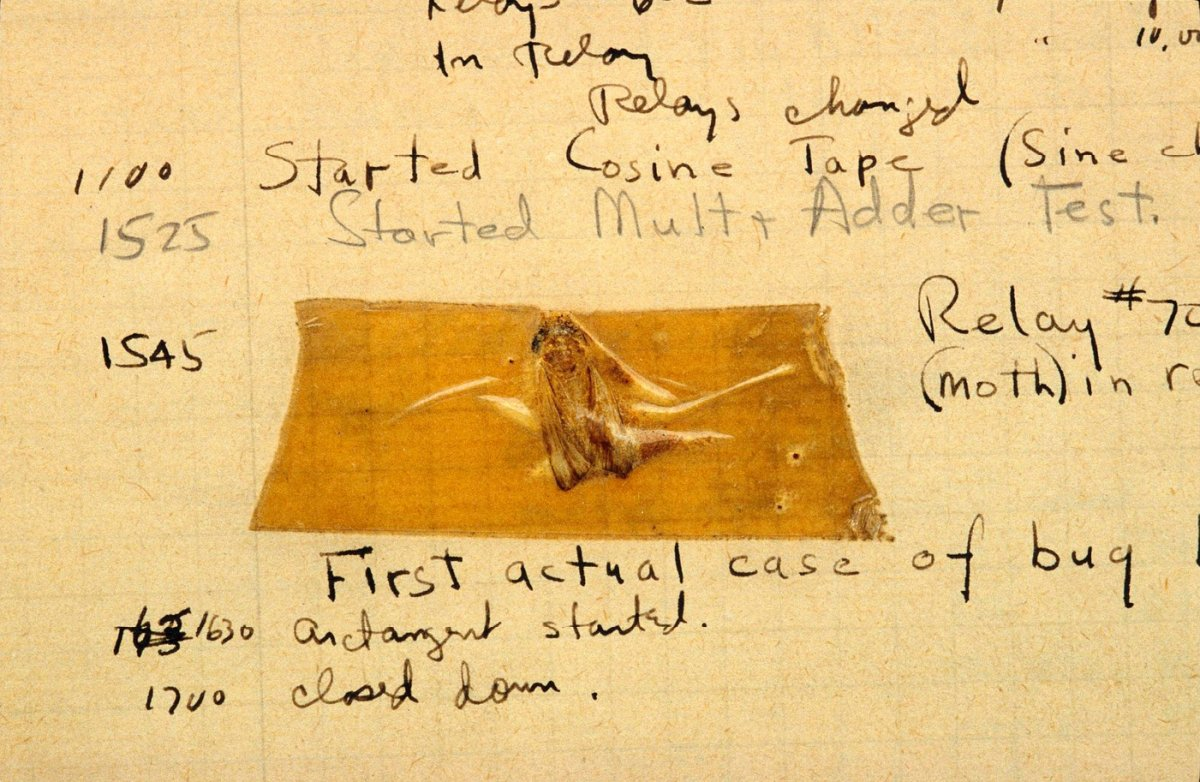
\includegraphics[width=0.85\textwidth]{figure/bug.jpg}
    \end{column}
  \end{columns}

  \begin{easylist}
    & 程序一次编写就能成功运行的概率很小,通常会有各种各样的错误需要调试,因此,
    掌握错误的调试方法非常重要。
  \end{easylist}
\end{frame}

\begin{frame}[fragile]{常用的调试方法}
  \begin{easylist}
    & 观察出错的提示信息
    & 利用print函数输出信息,观察输出结果和预期结果是否一致
    & 通过日志logging替代print
    & 利用assert断言
    & pdb
  \end{easylist}
\end{frame}

\subsubsection{利用print进行调试}
\begin{frame}[fragile]{利用print进行调试}
  \begin{python}
books = ['Python', 'XML', 'Information Retrieval']
for book in books:
    print(book)

print('Run here!') 
if book.price > 50:
    print('High price.')
  \end{python}

以上代码会抛出异常信息:

Traceback (most recent call last): \\
~~File "bug.py", line 5, in <module> \\
~~~~if book.price > 50: \\
AttributeError: 'str' object has no attribute 'price'\\

如果我们觉得前三行代码不太可能出问题,而问题很可能在后面,那我们可以在后面加入一
行print语句,观察程序能否正常运行到该位置,来缩小异常发生的范围
\end{frame}

\subsubsection{利用logging进行调试}
\begin{frame}[fragile]{利用logging进行调试}
  print()的结果默认输出到控制台上,不够灵活和方便,可以使用logging进行控制

  \begin{python}
import logging
logging.basicConfig(level=logging.INFO)

books = ['Python', 'XML', 'Information Retrieval']
for book in books:
    logging.info(book)

logging.debug('Run here!') 
if book.price > 50:
    logging.warn('High price.')
  \end{python}
\end{frame}

\subsubsection{assert调试}
\begin{frame}[fragile]{assert调试}
  assert断言用于判断给定的逻辑表达式是否成立,如果不成立,就会抛出AssertionError
  异常

\begin{python}
books = ['Python', 'XML', 'Information Retrieval']
assert len(books) == 3
\end{python}

启动Python解释器时可以用-O参数来关闭assert,此时的assert语句可看作是pass
\end{frame}

\subsubsection{pdb调试}
\begin{frame}[fragile]{pdb}
  Python的调试器,可以单步运行Python脚本,查看当前运行的代码,查看变量值

  bug.py: 
  \begin{python}
books = ['Python', 'XML', 'Information Retrieval']
for book in books:
    print(book)

if book.price > 50:
    print('High price.')
  \end{python}

  运行:pdb bug.py \\
  或者:python -m pdb bug.py

\end{frame}

\begin{frame}[fragile]{pdb}
  \begin{easylist}
    & n: 执行下一条语句
    & p xxx: 查看变量xxx的当前值
    & l: 列出
  \end{easylist}
\end{frame}

\begin{frame}[fragile]{pdb.set\_trace()}
  在可能出错的地方放置pdb.set\_trace(),程序运行到该条语句时,会暂停并进入pdb调试环
境,此时,可以用p指令查看变量,或者用c继续运行

  bug2.py: 
  \begin{python}
import pdb
books = ['Python', 'XML', 'Information Retrieval']
for book in books:
    print(book)

pdb.set_trace()
if book.price > 50:
    print('High price.')
  \end{python}
\end{frame}


\subsection{测试}

\begin{frame}[fragile]{测试}
  \begin{easylist}
    & 代码规范检查
    & 单元测试
  \end{easylist}
\end{frame}

\subsubsection{代码规范性检查工具}
\begin{frame}[fragile]{代码规范性检查工具}
  \begin{easylist}
    & pep8
    & pylint
    & pyflakes(略)
  \end{easylist}
\end{frame}

\begin{frame}[fragile]{pep8}
  \begin{easylist}
    & PEP: Python增强建议(Python Enhancement Proposals)
    && describe and document the way python language evolves. 
    && 完整的PEP索引列表:\url{https://www.python.org/dev/peps/}
    & PEP 8: Style Guide for Python Code
    && Pythonic way to write code
    && \url{https://www.python.org/dev/peps/pep-0008/}
  \end{easylist}
\end{frame}

\begin{frame}[fragile]{pep8示例}
  \begin{easylist}
    & 新建finder.py(源代码见下张幻灯片)
    & 打开终端,进入finder.py文件所在目录
    & 执行命令:\\
    ~~~~pep8~ finder.py
  \end{easylist}

  \begin{tcolorbox}[colback=green!5,colframe=green!50!black,title=输出结果]
    finder.py:3:1: E302 expected 2 blank lines, found 1 \\
    finder.py:19:1: W293 blank line contains whitespace \\
    finder.py:19:1: W391 blank line at end of file
  \end{tcolorbox}
\end{frame}


\begin{frame}[fragile]{finder.py源代码}
  \begin{lstlisting}[frame=single, language=Python,
    basicstyle=\scriptsize,numberstyle=\tiny\color{orange!90}\ttfamily,
    showstringspaces=false] 
# coding: utf-8

def first_index_of(sorted_name_list, name, start=0):
    '''获取排序列表sorted_name_list中指定名称元素的位置

    如果元素name在sorted_name_list中存在,则返回其下标,
    下标从0开始计数;如果不存在,则返回-1.

    >>> first_index_of([1,2,3], 1)
    0
    >>> first_index_of([1,2,3], 5)
    -1

    '''
    try:
        return sorted_name_list.index(name)
    except ValueError as e:
        return -1
  \end{lstlisting}
\end{frame}


\begin{frame}[fragile]{pylint}
  \begin{easylist}
    & \url{https://www.pylint.org/}
    && star your python code!
    && Coding Standard
    &&& checking line-code's length,
    &&& checking if variable names are well-formed according to your coding standard
    &&& checking if imported modules are used
    && Error detection
    &&& checking if declared interfaces are truly implemented
    &&& checking if modules are imported
    &&& and much more ...
  \end{easylist}
\end{frame}

\begin{frame}[fragile]{pylint}
  \begin{easylist}
    & 安装
    && sudo pip install pylint
    & 使用
    && pylint some\_file.py
    && 最终输出综合评分结果,例如:
  \end{easylist}

  \begin{tcolorbox}[colback=green!5,colframe=green!50!black,title=pylint输出结果片断]
    \textit{
      Global evaluation\\
      -----------------\\
      Your code has been rated at 8.38/10\\ }
  \end{tcolorbox}

\end{frame}

\subsubsection{单元测试}
% TODO: 参考Python高级编程 CH11
\begin{frame}[fragile]{单元测试}
  \begin{easylist}
    & 单元测试是用来对一个模块、一个函数或者一个类来进行正确性检验的测试工作。
    & TDD:Test-Driven Development
    && 敏捷开发中的一项常用技术和设计方法,即通过测试来推动整个开发的进行,在明确
    需要开发的功能后,首先思考如何对功能进行测试,进而完成测试用例代码的编写,然后
    实现具体产品功能,满足之前设计的测试用例。
    & Python的单元测试模块
    && unittest:最初由Steve Purcell编写,以前叫PyUnit
    && doctest: 一个依赖于Python的doc字符串的测试工具
    & 第三方提供的单元测试工具(略)
    && nose
    && py.test
  \end{easylist}
\end{frame}

\begin{frame}[fragile]{unittest}
  \begin{easylist}
    & 类似于Java中的JUnit
    & 提供了一个TestCase基类,该基类拥有一个用来验证输入输出的方法集合
    & 示例
    && 假设有一个工具方法模块utils.py, 里面包含一个求平均数的函数average
    && 现在需要编写对应的单元测试
  \end{easylist}
\end{frame}


\begin{frame}[fragile, allowframebreaks]{test\_utils.py代码清单}
  \lstinputlisting[keywordstyle=\ttfamily]{src/ch8/test_utils.py}

  运行``python test\_utils.py''进行测试
\end{frame}


\begin{frame}[fragile]{utils.py代码清单}
  \lstinputlisting[keywordstyle=\ttfamily]{src/ch8/utils.py}  
\end{frame}

\begin{frame}[fragile]{doctest}
  \begin{easylist}
    & doctest:在docstring中编写测试代码
    & 优点:
    && 可以通过示例创建文档和测试
    && 文档示例总是最新的
    & 注意:
    && doctest应该只被用于在文档中提供人类可读的示例
    && 帮助文档有可能因为加入过多的测试代码而破坏了其可阅读性
    & 例子:
    && 为上例中的utils.py中的average函数添加docstring
  \end{easylist}
\end{frame}

\begin{frame}[fragile, allowframebreaks]{utils2.py代码清单}
  \lstinputlisting[keywordstyle=\ttfamily]{src/ch8/utils2.py}  
\end{frame}

\begin{frame}[fragile]{第三方测试框架}
  \begin{easylist}
    & unittest过于僵化,不易扩展
    && 必须继承TestCase
    && 必须使用TestCase本身所提供的断言方法
    && 测试方法名称前需要加test
    && $\cdots$
    & 全部使用doctest替代单元测试会破坏文档的可阅读性
    && $\cdots$
    & 提出了一些第三方测试框架
    && nose
    && py.test
  \end{easylist}
\end{frame}

\begin{frame}[plain]{}
  \begin{center}
    ~ \\
    \Huge ---END---
  \end{center}
\end{frame}

\section{Web处理}

\begin{frame}[fragile]{Web服务器}
  \begin{easylist} \easyitem
    & 最简单的Python Web服务器
    & Flask
  \end{easylist}
\end{frame}

\begin{frame}[fragile]{Simple Http Server}
  \begin{easylist}

    & 最轻便的Web服务器\footnote{参数m的作用参考:
      \url{http://www.tuicool.com/articles/jMzqYzF}}:

    & 启动方式:
    && python -m http.server
  \end{easylist}
\end{frame}

\begin{frame}[fragile]{Flask}
  \begin{easylist}
    & Flask是一种简便的基于Python语言的Web应用程序开发框架
    && Flask is a microframework for Python based on Werkzeug, Jinja 2 and good intentions. And before you ask: It's BSD licensed!
    & 相关中文文档可在线参考:
    &&
    \scriptsize{\url{http://dormousehole.readthedocs.io/en/latest/quickstart.html}
    }
    & 安装:
    && pip install Flask
    & 文档
    && http://flask.pocoo.org/docs/0.10/.latex/Flask.pdf
  \end{easylist}
\end{frame}


\begin{frame}[fragile]{Flask简单例子}
  \lstinputlisting[keywordstyle=\ttfamily]{src/web/flask1.py}
\end{frame}

\begin{frame}[fragile, allowframebreaks]{Flask简单例子}
  \lstinputlisting[keywordstyle=\ttfamily]{src/web/flask2.py}
\end{frame}

\begin{frame}[fragile]{练习}
  实现一个Web程序,在网页上输入一个url地址,提交后,通过浏览器显示该地址所包含的所有图片。
\end{frame}


\begin{frame}[fragile]{科研人员在线社交媒体行为分析}
  \begin{easylist}
    & 编写一个Web应用程序,记录每个高校在社交媒体上的活动信息
    && 第一步完成基本信息的收集管理
    & 基本信息包括
    && 学校名称, 学院, 专业, 姓名, 性别, 出生年, 简介, 微博UID, 微博注册日期, 最
    后访问日期
  \end{easylist}

  \begin{easylist}
    & 基本信息管理功能:
    && 基本信息录入
    && 重复检测(根据学校、学院、姓名判断重复,或者根据微博UID判断重复)
    && 检索统计:
  \end{easylist}
\end{frame}

%%% Local Variables:
%%% mode: latex
%%% TeX-master: "../python"
%%% End:

\end{document}


%%% Local Variables:
%%% mode: latex
%%% TeX-master: t
%%% End:
